% Preamble
\documentclass{hnu}

% Packages
\usepackage{amsmath}
\usepackage{algorithm}
\usepackage{algorithmic}
\usepackage{booktabs}
\usepackage{graphicx}
\usepackage{overpic}
\usepackage{fontspec}
\usepackage{multirow}
\usepackage{tikz}
\usetikzlibrary{shapes.geometric, arrows.meta, positioning, fit, backgrounds, calc}
\usepackage{pgfplots}
\usepackage{amssymb}
\usepackage{pkgs/cover}
\usepackage{pkgs/copyright}
\usepackage{pkgs/tocloflot}
\usepackage{pkgs/bibliography}
\usepackage{pkgs/appendix}

% Float layout tuning
\renewcommand{\topfraction}{0.9}
\renewcommand{\bottomfraction}{0.8}
\renewcommand{\textfraction}{0.08}
\renewcommand{\floatpagefraction}{0.75}
\setlength{\floatsep}{8pt plus 2pt minus 2pt}
\setlength{\textfloatsep}{10pt plus 2pt minus 2pt}
\setlength{\intextsep}{8pt plus 2pt minus 2pt}

% Document
\begin{document}
    \createCover % 封面

    \frontmatter
    \createCopyright % 版权

    % ========================================摘要部分
    \begin{abstractCN}
    服务器日志记录了系统运行过程中的事件状态、错误信息和组件行为，是开展故障诊断和异常检测的重要数据来源。针对原始日志格式不统一、动态参数较多、事件序列具有非规则时间间隔以及异常样本比例较低等问题，本文设计并实现了一种基于日志分析和 Liquid 架构的服务器异常检测系统。系统首先对原始日志进行字段抽取、时间排序、文本清洗和动态参数归一化处理；随后将非结构化日志正文解析为日志模板和事件 ID，并以时间窗口为单位构建事件频次、事件序列和相邻事件时间间隔等联合特征；最后使用 Liquid 模型对窗口级日志状态进行建模，并基于验证集选择异常判定阈值。实验部分以 BGL 数据集为主要测试对象，并引入 HDFS 数据集进行辅助对比。实验结果表明，本文系统能够完成从原始日志输入到异常结果输出的完整流程，在 BGL 测试集上取得 Precision 为 0.945、Recall 为 0.932、F1 值为 0.938 的检测结果。本文工作验证了将日志模板、统计频次、事件顺序和时间间隔信息结合用于服务器异常检测的可行性。

    \keywordsCN 日志分析；服务器异常检测；日志解析；特征工程；Liquid 架构；时序建模
\end{abstractCN}

\begin{abstractENG}
    Server logs record runtime events, error messages, and component behaviors, and therefore provide an important data source for fault diagnosis and anomaly detection. To address the problems of inconsistent log formats, numerous dynamic parameters, irregular time intervals between log events, and imbalanced anomaly samples, this thesis designs and implements a log-based server anomaly detection system using a Liquid architecture. The system first extracts key fields from raw logs, sorts log records by timestamp, cleans log messages, and normalizes dynamic parameters. It then parses unstructured log messages into log templates and event IDs, and constructs joint features based on event frequency, event sequence, and time interval within each time window. Finally, a Liquid model is used to model window-level log states, and the anomaly threshold is selected on the validation set. The experiments use the BGL dataset as the main benchmark and introduce the HDFS dataset for auxiliary comparison. The experimental results show that the proposed system can complete the end-to-end workflow from raw log input to anomaly output, achieving a Precision of 0.945, a Recall of 0.932, and an F1-score of 0.938 on the BGL test set. This work verifies the feasibility of combining log templates, statistical frequency, event order, and time-interval information for server anomaly detection.

    \keywordsENG Log Analysis; Server Anomaly Detection; Log Parsing; Feature Engineering; Liquid Architecture; Time Series Modeling
\end{abstractENG}

    % ========================================摘要部分

    \createTOC % 目录
    \createLOF % 插图索引
    \createLOT % 附表索引

    \mainmatter
    % ========================================正文部分
    \chapter{绪论}
\vspace{7pt}

\section{课题背景}

随着互联网服务、云计算平台和分布式系统的快速发展，服务器系统已经成为企业业务承载、数据存储、在线交易、智能运维和网络安全防护的重要基础设施。因此，如何从海量运行数据中及时发现系统异常状态，已经成为可靠性工程、智能运维和异常检测领域的重要研究问题\cite{chandola2009anomaly,he2016experience}。

服务器日志是系统运行过程中自动生成的重要文本数据，记录了服务器在不同时间点发生的事件、状态变化、错误信息、用户行为以及进程调用过程。因此，基于日志分析实现服务器异常状态检测，对于故障预警、风险控制和系统维护具有重要价值。\cite{oliner2007supercomputers,xu2009detecting}\cite{chandola2009anomaly,he2016experience}\cite{vaarandi2015logcluster,du2016spell,he2017drain,zhu2019tools}\cite{du2017deeplog,meng2019loganomaly,guo2021logbert}\cite{hochreiter1997lstm}\cite{vaswani2017attention}\cite{he2009imbalanced,saito2015precision}\cite{hasani2021liquid,chen2018neuralode}


\section{课题研究意义}

本课题围绕服务器日志异常检测问题，设计并实现一种基于日志分析与 Liquid 架构的服务器异常检测系统。系统从原始日志数据出发，依次完成日志预处理、日志解析、特征工程、模型训练、阈值优化和异常判别等步骤，最终实现对服务器异常状态的自动识别。

首先，本课题有助于提升服务器运维的自动化与智能化水平。通过构建自动化日志异常检测系统，可以在海量日志中快速发现潜在异常模式，减少人工排查成本，使运维人员能够更加及时地定位故障和处理风险。\cite{xu2009detecting,he2016experience}\cite{saito2015precision}


\section{国内外研究现状}

日志异常检测是智能运维领域的重要研究方向之一。随着系统规模不断扩大，国内外学者围绕日志数据集建设、日志解析、日志特征表示和异常检测模型等方面开展了大量研究。

在日志数据集与日志分析基础研究方面，Oliner 和 Stearley 对多类超级计算机系统日志进行了系统研究，指出系统日志能够反映大规模计算系统的运行状态和故障特征\cite{oliner2007supercomputers}。Xu 等通过挖掘控制台日志检测大规模系统问题，证明了从日志中提取事件模式和统计特征进行异常检测的可行性\cite{xu2009detecting}。\cite{zhu2023loghub}\cite{vaarandi2015logcluster}\cite{du2016spell}\cite{he2017drain}\cite{zhu2019tools}\cite{mikolov2013efficient,devlin2019bert}\cite{du2017deeplog}\cite{scholkopf2001estimating,liu2008isolation}\cite{meng2019loganomaly}\cite{guo2021logbert}\cite{he2009imbalanced,saito2015precision}\cite{vaswani2017attention,guo2021logbert}\cite{chen2018neuralode}\cite{hasani2021liquid,hasani2022closedform}\cite{lechner2020neural}


\section{本文主要研究内容}

本文以服务器日志数据为研究对象，围绕日志异常检测问题，设计并实现一个基于日志分析与 Liquid 架构的服务器异常检测系统。本文的主要研究内容包括以下几个方面。

\subsection{日志数据预处理}

原始服务器日志通常存在格式不统一、字段冗余、噪声信息较多和数据缺失等问题。本文首先对日志数据库中的原始数据进行清洗与规范化处理，包括日志数据读取、无效字段过滤、时间戳统一转换、重复日志去除以及特殊字符清理等。

\subsection{基于规则与正则表达式的日志解析}

针对预处理后的非结构化日志文本，本文设计日志解析模块。该模块通过规则和正则表达式识别日志中的动态参数，例如 IP 地址、端口号、时间字段、进程编号、内存地址和数字变量等，并将其替换为统一占位符，从而提取代表核心语义的固定日志模板。\cite{vaarandi2015logcluster,he2017drain,zhu2019tools}

\subsection{面向连续时序的特征工程构建}

为适配 Liquid 模型的连续时间建模特点，本文设计联合特征构建方法。通过这种方式，模型输入同时包含局部统计分布、事件顺序和时间间隔信息，有助于更全面地描述服务器运行状态。

\subsection{基于 Liquid 架构的模型训练与动态阈值寻优}

针对传统离散时序模型难以充分利用非规则日志时间间隔的问题，本文采用 Liquid 架构构建异常检测核心模型。模型以日志窗口特征序列为输入，通过连续时间动态机制学习服务器正常运行状态下的状态演化规律，并输出异常评分或异常概率。\cite{he2009imbalanced,saito2015precision}

\subsection{异常检测系统设计、实现与实验验证}

在算法研究的基础上，本文实现一套端到端服务器日志异常检测系统。系统整合日志读取、数据清洗、模板解析、特征工程、模型训练、动态阈值选择、异常推断和结果输出等模块，实现数据自动化流转和异常状态识别。

\section{本文主要贡献与创新点}

针对现有服务器日志异常检测方法在非规则时序建模、类别不平衡处理和工程落地方面的不足，本文开展了模型设计与系统实现工作，主要贡献与创新点如下。

\begin{enumerate}
    \item \textbf{探索了 Liquid 架构在服务器日志异常检测中的应用。} 本文将基于连续时间动态系统的 Liquid 架构引入日志异常检测任务，利用其对时间间隔和输入变化的动态响应能力，刻画服务器日志在非规则采样条件下的状态演化过程，为离散日志序列建模提供了新的实现思路。
    
    \item \textbf{提出了一种融合统计频次与事件序列的联合特征构建方法。} 针对单一特征表达能力有限的问题，本文在时间窗口机制下同时构建事件频次分布特征和事件顺序编码特征，使模型既能够感知局部事件密度变化，也能够保留日志事件之间的时序依赖关系。
    
    \item \textbf{设计了面向类别不平衡问题的动态阈值寻优策略。} 针对真实服务器日志中异常样本占比较低的问题，本文基于验证集 Precision-Recall 曲线选择异常判定阈值，避免简单采用固定阈值造成误报或漏报偏高，从而提升模型在不平衡数据场景下的综合检测效果。
    
    \item \textbf{实现并验证了一套端到端自动化日志异常检测系统。} 本文打通了从日志读取、清洗、解析、特征构建，到模型训练、异常推断和结果输出的完整流程，并在公开日志数据集上进行实验验证，证明了系统在服务器异常检测任务中的可行性和工程应用价值。
\end{enumerate}

\section{本文组织结构}

本文共分为六章，各章节内容安排如下。

\textbf{第一章 绪论。} 主要阐述服务器日志异常检测的课题背景与研究意义，梳理国内外在日志解析、特征表示、异常检测模型和连续时间建模方面的研究现状，指出现有方法的不足，并概述本文的主要研究内容、贡献与论文组织结构。

\textbf{第二章 相关理论与关键技术。} 介绍服务器日志的数据特性与分析难点，回顾日志预处理、日志解析、特征工程和异常检测的常用方法；重点阐述深度学习时序模型、Liquid 架构以及 Liquid Time-Constant Networks 的基本思想，为后续系统设计与模型实现奠定理论基础。

\textbf{第三章 系统需求分析与总体设计。} 从实际运维应用场景出发，对系统进行功能需求和非功能需求分析，论证系统建设可行性；随后提出系统总体架构，明确数据层、处理层、模型层和输出层的模块划分，并设计核心数据流转过程和数据库结构。

\textbf{第四章 系统实现。} 详细描述系统各功能模块的具体实现过程，包括日志读取与清洗、正则表达式驱动的日志解析、基于时间窗口的特征工程构建、Liquid 异常检测模型的训练与推断，以及动态阈值判定和异常检测结果输出逻辑。

\textbf{第五章 系统测试与实验分析。} 基于公开服务器日志数据集对本文系统进行功能测试和性能评估，展示模型训练过程、异常评分变化和检测结果，并使用准确率、精确率、召回率、F1 值等指标与相关基线方法进行对比分析；同时对输入序列长度、时间窗口大小和判定阈值等关键因素进行讨论。

\textbf{第六章 总结与展望。} 对全文研究工作进行总结，归纳本文取得的主要成果；同时分析当前系统在复杂日志泛化、深层语义利用和流式实时处理方面存在的不足，并提出后续改进方向和研究展望。
    \chapter{理论技术}
\vspace{7pt}

\section{日志概述}

服务器日志是系统在运行过程中产生的事件记录，通常包含时间、节点、组件、日志级别和日志正文等信息。日志既记录正常执行过程，也记录异常告警、错误堆栈和资源访问情况，是分析服务器运行状态的重要数据来源。与结构化监控指标相比，日志具有更丰富的语义信息，但也存在格式不统一、噪声较多和动态参数复杂等问题\cite{oliner2007supercomputers,xu2009detecting}。

服务器日志通常具有以下特点。

\begin{enumerate}
    \item \textbf{规模较大。} 服务器在持续运行过程中会产生大量日志，高并发服务、分布式部署和多节点集群会进一步增加日志规模。
    \item \textbf{格式多样。} 不同组件和程序模块输出的日志格式并不一致，同一系统内部也可能同时存在结构化、半结构化和自由文本日志。
    \item \textbf{时序性。} 日志按照时间顺序产生，事件之间的先后关系能够反映系统执行路径和故障传播过程。
    \item \textbf{采样不均匀。} 日志不是等间隔产生的数据。系统平稳运行时日志较为稀疏，异常发生时可能出现短时间高密度输出。
    \item \textbf{类别不平衡。} 正常日志通常占绝大多数，异常日志数量相对较少，模型容易偏向多数类。
\end{enumerate}

上述特点决定了日志异常检测需要先将原始文本转换为结构化表示，再结合统计、序列和时间特征进行建模。

\section{日志预处理}

原始日志不能直接用于模型训练。日志预处理的目标是消除无效字段和格式差异，保留与异常检测相关的信息，并为后续日志解析和特征构建提供规范输入。

\subsection{数据清洗}

日志数据清洗主要包括空值处理、重复记录过滤、异常字符清理和无关字段筛选。空值处理用于去除时间戳或日志正文缺失的记录；重复记录过滤用于减少重复输出对频次统计的干扰；异常字符清理用于统一空白符、控制字符和无意义符号；无关字段筛选用于降低输入维度。清洗过程不应改变异常标签和时间戳等监督学习所需字段。

\subsection{时间标准化}

日志具有时间属性，时间戳标准化是时序建模的基础。设原始日志集合为
\begin{equation}
    L=\{l_1,l_2,\cdots,l_n\},
\end{equation}
其中第 $i$ 条日志可表示为 $l_i=(t_i,c_i,m_i)$，$t_i$ 为时间戳，$c_i$ 为结构化字段，$m_i$ 为日志正文。经过时间排序后得到
\begin{equation}
    L'=sort(L,t_i).
\end{equation}
排序后的日志能够保留事件先后关系，并为时间窗口划分和相邻事件时间间隔计算提供依据。

\subsection{级别处理}

日志级别通常包括 INFO、WARN、ERROR、DEBUG 和 FATAL 等。日志级别能够反映事件严重程度，但不能简单等同于异常标签。例如，单条 ERROR 日志可能被自动恢复，而多个 INFO 事件的异常顺序也可能提示系统状态异常。因此，日志级别适合作为辅助特征，而不宜作为唯一判定规则。

\section{日志解析}

日志解析的目标是将非结构化日志正文转换为结构化事件。日志正文通常由固定模板和动态参数组成，其中固定模板描述事件语义，动态参数描述运行时变量。若不进行解析，同一事件会因不同 IP、端口、路径或编号被视为不同文本，导致模型输入空间膨胀。

\subsection{日志模板}

例如，以下两条日志的动态参数不同，但表示同一类连接失败事件。

\begin{verbatim}
2025-03-01 10:12:03 ERROR Failed to connect to 192.168.1.10:8080
2025-03-01 10:12:08 ERROR Failed to connect to 192.168.1.15:8080
\end{verbatim}

经过模板化处理后，可表示为
\begin{verbatim}
Failed to connect to <*>:<*>
\end{verbatim}
其中 \texttt{<*>} 表示被归一化的动态参数。设日志解析函数为 $P(\cdot)$，日志正文 $m_i$ 可映射为事件 ID：
\begin{equation}
    e_i=P(m_i).
\end{equation}

\subsection{解析方法}

常见日志解析方法包括规则方法、聚类方法、树结构方法和学习方法。规则方法依赖人工设计正则表达式，实现成本低，适合格式稳定的日志。聚类方法根据文本相似度或词项分布抽取模板，能够减少人工规则设计，但在大规模日志上计算成本较高。树结构方法通过分层匹配提升解析效率，适合在线日志处理。学习方法能够自动提取日志结构，但通常需要较多训练样本和额外计算资源\cite{zhu2019tools,du2016spell,he2017drain}。

本文面向毕业论文系统实现和实验验证，采用规则与正则表达式结合的解析方式。该方式实现过程明确，便于复现，并便于在后续实验中解释模板生成结果。

\section{特征工程}

日志解析后得到事件序列，但事件 ID 仍需转换为模型可处理的数值特征。本文从事件频次、事件顺序和时间间隔三个角度构建特征。

\subsection{事件频次}

事件频次特征用于统计时间窗口内不同事件模板的出现次数。已有系统日志研究表明，事件计数和模板分布能够反映系统在局部时间范围内的运行状态。设模板集合为 $V=\{v_1,v_2,\cdots,v_k\}$，第 $j$ 个时间窗口为 $W_j$，其频次向量表示为
\begin{equation}
    X_j=[x_{j1},x_{j2},\cdots,x_{jk}],
\end{equation}
其中 $x_{jp}$ 表示模板 $v_p$ 在窗口 $W_j$ 中出现的次数。该特征能够反映局部事件分布变化，适合捕捉异常爆发导致的频次突增。

\subsection{日志序列}

事件频次无法表达事件先后顺序。对于服务器日志而言，某些异常并不表现为单个事件异常，而表现为事件组合顺序异常。因此，本文将窗口内日志按照时间排序后构造事件序列\cite{du2017deeplog,meng2019loganomaly}
\begin{equation}
    S_j=\{e_{j1},e_{j2},\cdots,e_{js}\}.
\end{equation}
当窗口内事件数量不足固定长度时使用补齐标记；当事件数量超过固定长度时保留最近的连续片段，以保证输入维度一致。

\subsection{时间间隔}

日志事件之间的真实时间间隔能够描述系统状态变化速度。对于非规则采样序列，连续时间建模能够避免将不同实际时间跨度的事件间隔简单视为相同时间步。设连续事件 $e_{i-1}$ 和 $e_i$ 的时间戳分别为 $t_{i-1}$ 和 $t_i$，其时间间隔定义为\cite{rubanova2019latentode}
\begin{equation}
    \Delta t_i=t_i-t_{i-1}.
\end{equation}
异常爆发时，多个事件可能在短时间内密集出现；平稳运行时，相邻日志间隔可能较长。将 $\Delta t_i$ 显式输入模型，有助于模型区分事件顺序相同但发生节奏不同的样本。

\subsection{嵌入表示}

事件 ID 是离散变量，直接使用整数编号可能引入不存在的大小关系。为增强模型表达能力，本文使用嵌入层将事件 ID 映射为连续向量：
\begin{equation}
    h_i=Embedding(e_i), \quad h_i\in\mathbb{R}^{d}.
\end{equation}
嵌入向量与频次特征、时间间隔特征拼接后形成联合输入。

\section{异常检测}

异常检测的目标是识别与正常运行模式存在差异的样本。在服务器日志场景中，异常可以表现为单条严重错误日志，也可以表现为一段时间内事件分布、事件顺序或时间节奏的异常变化。

\subsection{异常类型}

本文将日志异常概括为三类。

\begin{enumerate}
    \item \textbf{点异常。} 单条日志本身具有异常含义，例如严重故障或系统崩溃信息。
    \item \textbf{上下文异常。} 日志事件本身并不罕见，但在特定时间或特定运行阶段出现时不符合系统状态。
    \item \textbf{序列异常。} 多条日志组合后的顺序、频率或时间间隔偏离正常模式。
\end{enumerate}

本文重点关注窗口级异常检测，即判断某一时间窗口或日志轨迹是否处于异常状态。

\subsection{类别不平衡}

服务器日志异常样本比例通常较低。若模型简单地将全部样本预测为正常，可能获得较高准确率，但无法识别真正异常。因此，模型评价不能只依赖 Accuracy，还需要结合 Precision、Recall 和 F1 值进行分析\cite{he2009imbalanced,saito2015precision}。

\subsection{评价指标}

在二分类检测中，Precision 和 Recall 定义为
\begin{equation}
    Precision=\frac{TP}{TP+FP}, \quad Recall=\frac{TP}{TP+FN}.
\end{equation}
F1 值为二者的调和平均数：
\begin{equation}
    F1=\frac{2\times Precision\times Recall}{Precision+Recall}.
\end{equation}
其中，TP 表示异常样本被正确识别为异常，FP 表示正常样本被误报为异常，FN 表示异常样本被漏报。本文模型输出连续异常评分，最终类别由阈值决定。为减少固定阈值带来的偏差，本文在验证集上选择使 F1 值较优的阈值。

\section{Liquid 架构}

Liquid 架构是一类连续时间递归神经网络。与普通离散时序模型不同，Liquid 模型通过状态演化方程描述隐藏状态随输入和时间变化的过程，适合处理不规则采样序列\cite{chen2018neuralode,hasani2021liquid}。

以 Liquid Time-Constant Networks 为例，其单个神经元状态可抽象表示为
\begin{equation}
    \frac{dx(t)}{dt}=-\left[\frac{1}{\tau}+f(I(t),x(t),\theta)\right]x(t)+f(I(t),x(t),\theta)A,
    \label{eq:ltc_core}
\end{equation}
其中，$x(t)$ 表示状态变量，$\tau$ 表示基础时间常数，$I(t)$ 表示输入特征，$A$ 表示静息状态，$f(\cdot)$ 表示可学习的非线性函数。由式 \ref{eq:ltc_core} 可见，模型状态变化不仅依赖当前输入，也受到时间常数影响。

在本文系统中，Liquid 架构与日志异常检测的结合方式如下。首先，日志事件 ID 经嵌入层映射为连续向量；其次，系统将时间间隔作为显式输入，使模型能够感知日志产生节奏；最后，模型根据窗口内事件序列输出异常评分，并通过验证集阈值完成异常判定。该机制使模型能够同时利用事件语义、事件顺序和非规则时间信息。

\section{本章小结}

本章围绕服务器日志异常检测所需理论和技术进行了说明。首先分析了服务器日志的规模、格式、时序、采样和类别分布特征，明确了原始日志需要经过清洗、解析和特征构建后才能用于模型训练。其次，介绍了日志模板、动态参数替换和事件 ID 映射等日志解析思想，说明了将非结构化日志转换为结构化事件序列的必要性。随后，本章从事件频次、事件顺序、时间间隔和嵌入表示四个方面说明了日志特征工程方法，并给出了异常检测任务中常用的评价指标。最后，本章介绍了 Liquid 架构的连续时间建模思想，说明了其与服务器日志非规则时间间隔特征之间的对应关系。

本章内容为后续系统设计提供理论基础。第三章将在本章基础上进一步给出系统总体架构、关键模块和算法流程；第四章将说明这些理论与设计如何落实为可运行的系统实现；第五章将通过实验验证相关设计的有效性。

需要强调的是，本文所采用的理论和技术并非相互独立。日志解析决定事件 ID 的稳定性，事件 ID 决定序列建模的输入空间，时间窗口决定样本粒度，时间间隔决定连续时间建模的信息来源，评价指标决定阈值选择方向。若其中任一环节设计不合理，都会影响最终异常检测效果。因此，后续章节将按照数据流顺序展开，使每个模块的设计目的、实现方式和实验验证形成对应关系。

    \chapter{系统需求分析与总体设计}
\vspace{7pt}

\section{本章引言}

上一章从日志数据特性、日志解析、特征工程、异常检测评价指标以及 Liquid 架构等方面介绍了本文研究所需的理论基础。因此，本章围绕“结构化解析—连续时序特征构建—Liquid 动态建模—动态阈值判定”的技术路线，对基于日志分析的服务器异常检测系统进行需求分析与总体设计。\cite{oliner2007supercomputers,xu2009detecting,he2021survey}

本章首先分析系统的应用场景、功能需求、非功能需求和可行性；随后设计系统总体架构与核心模块；

\section{系统需求与可行性分析}

\subsection{系统应用场景}

服务器在运行过程中持续产生大量日志，日志中记录了服务调用、资源状态、错误信息和系统告警等内容。当服务器出现异常时，日志通常会出现局部密度升高、特定模板频繁出现、关键事件缺失或事件顺序异常等现象\cite{oliner2007supercomputers,xu2009detecting,he2016experience}。\cite{chandola2009anomaly,he2021survey,landauer2023survey}

本文系统面向服务器智能运维场景，主要完成以下任务：第一，对原始日志进行清洗、解析和结构化管理；第二，基于时间窗口构建事件频次、事件序列和时间间隔等联合特征；

\subsection{功能需求分析}

根据系统目标，本文系统划分为日志输入、日志预处理、日志解析、特征工程、模型训练、异常检测和结果输出七类功能；这一流程与自动化日志分析中“清洗—解析—表示—检测”的典型技术链路保持一致\cite{zhu2019tools,he2021survey}。各功能需求如表 \ref{tab:function_requirements_new} 所示。

\begin{table}[htbp]
    \centering
    \caption{系统功能需求表}
    \label{tab:function_requirements_new}
    \begin{tabular}{p{3cm} p{9cm}}
        \hline
        功能模块 & 功能说明 \\
        \hline
        日志输入模块 & 读取日志文件或日志数据库，提取时间戳、节点、组件、日志级别、日志内容和原始标签等字段，并按时间升序组织日志。 \\
        日志预处理模块 & 完成缺失字段过滤、重复记录去除、时间格式统一、动态噪声清理和关键字段规范化。 \\
        日志解析模块 & 识别日志中的动态参数，生成日志模板，将非结构化日志映射为事件 ID 序列，并维护模板映射表。 \\
        特征工程模块 & 基于时间窗口生成样本，构建事件频次、事件序列、时间间隔和窗口标签，形成 Liquid 模型输入张量。 \\
        模型训练模块 & 使用训练集更新 Liquid 模型参数，使用验证集选择最优模型和异常判定阈值。 \\
        异常检测模块 & 对待检测日志执行与训练阶段一致的处理流程，加载模型和阈值，输出异常评分与分类结果。 \\
        结果输出模块 & 保存异常窗口、异常评分、预测标签、真实标签和评价指标，为系统展示和实验分析提供数据。 \\
        \hline
    \end{tabular}
\end{table}

\subsection{非功能需求分析}

为保证系统具有实际应用价值，本文从准确性、效率、稳定性、可扩展性和可维护性五个方面提出非功能需求。

\begin{enumerate}
    \item \textbf{准确性需求。} 系统以 Precision、Recall 和 F1 值作为主要评价指标，重点降低异常漏报，同时控制误报数量。由于日志异常检测存在类别不平衡问题，系统不使用固定 0.5 阈值，而是在验证集上进行阈值校准\cite{he2009imbalanced,saito2015precision}。
    \item \textbf{效率需求。} 系统在预处理和特征工程阶段采用批量处理方式，在模型阶段使用固定长度序列和轻量级 Liquid 隐藏层，降低海量日志训练与检测的计算开销。
    \item \textbf{稳定性需求。} 系统对空窗口、缺失字段、未知日志模板和异常时间戳进行统一处理，避免单条异常数据破坏整体检测流程。
    \item \textbf{可扩展性需求。} 系统通过字段映射、模板映射和特征配置支持不同日志数据集，例如 BGL 和 HDFS。新增日志格式时，只需调整字段抽取和解析规则，后续模型输入结构保持一致。
    \item \textbf{可维护性需求。} 系统采用模块化设计，各模块之间通过结构化数据表和统一特征接口连接，便于替换日志解析算法、调整特征组合或扩展检测模型。
\end{enumerate}

\subsection{系统可行性分析}

从技术角度看，本文系统所需的数据清洗、正则解析、特征构建和深度学习训练均可基于 Python、Pandas、NumPy 和 PyTorch 等工具实现\cite{mckinney2010data,harris2020array,paszke2019pytorch}。Liquid 架构虽然需要对隐藏状态进行连续时间建模，但本文将输入样本限制为固定长度日志窗口，并采用轻量级隐藏层和 Euler 数值求解方式，因此计算复杂度处于可控范围。

从经济角度看，本文系统主要基于公开日志数据集和开源软件完成开发与实验，不依赖专用商业平台，普通实验服务器即可满足模型训练与测试需求。从操作角度看，系统按照日志读取、预处理、解析、特征工程、训练和检测的顺序组织流程，运行过程清晰，具备较好的操作可行性。

\section{系统总体设计}

\subsection{设计目标}

本文系统的总体目标是构建端到端的服务器日志异常检测流程，将原始日志转化为可用于连续时序建模的结构化样本，并输出可靠的异常检测结果。具体目标如下：

\begin{enumerate}
    \item 对原始日志进行规范化处理，保留时间戳、节点、日志级别、组件、内容和标签等关键信息；
    \item 将非结构化日志文本解析为日志模板和事件 ID，降低文本维度并保留事件语义\cite{jiang2008ael,he2017drain,zhu2019tools}；
    \item 在时间窗口内同时提取事件频次、事件顺序和相邻事件时间间隔，形成联合特征表示；
    \item 利用 Liquid 架构建模日志状态在连续时间上的动态演化过程\cite{chen2018neuralode,hasani2021liquid,hasani2022closedform}；
    \item 通过验证集动态选择异常阈值，并在测试阶段输出异常评分、预测标签和评价指标。
\end{enumerate}

\subsection{总体架构设计}

系统总体架构由数据层、处理层、模型层和输出层组成。数据层负责存储原始日志、清洗日志、模板映射、特征样本、模型配置和检测结果；

系统整体流程如图 \ref{fig:system_architecture_new} 所示。与单向流水线不同，本文将系统划分为离线训练流程和在线检测流程。\cite{he2016experience,zhu2019tools}

\begin{figure}[htbp]
    \centering
    \begin{tikzpicture}[
        node distance=1cm and 0.5cm,
        % 定义离线阶段的矩形框样式
        box/.style={rectangle, draw=blue!70!black, fill=blue!5, thick, rounded corners=2mm, minimum height=0.9cm, minimum width=2.6cm, align=center, font=\small},
        % 定义在线阶段的矩形框样式
        onlinebox/.style={rectangle, draw=green!70!black, fill=green!5, thick, rounded corners=2mm, minimum height=0.9cm, minimum width=2.6cm, align=center, font=\small},
        % 定义实线箭头样式
        arrow/.style={-{Stealth[scale=1.2]}, thick, draw=black!80},
        % 定义虚线箭头样式
        darrow/.style={-{Stealth[scale=1.2]}, thick, dashed, draw=black!80},
        % 定义背景分组框样式
        groupbox/.style={rectangle, draw=black!50, dashed, thick, inner sep=12pt, rounded corners=2mm}
    ]

    % ---------------- 离线训练阶段 (第一行) ----------------
    \node[box] (d1) {历史日志数据};
    \node[box, right=of d1] (d2) {预处理};
    \node[box, right=of d2] (d3) {日志解析};
    \node[box, right=of d3] (d4) {联合特征构建};

    \draw[arrow] (d1) -- (d2);
    \draw[arrow] (d2) -- (d3);
    \draw[arrow] (d3) -- (d4);

    % ---------------- 划分数据集 (第二行) ----------------
    \path (d1.west) -- (d4.east) coordinate[midway] (center_top);
    \node[box, below=0.8cm of center_top, minimum width=12.2cm] (split) {按时间顺序划分训练集、验证集和测试集};
    
    \draw[arrow] (d4.south) -- (d4.south |- split.north);

    % ---------------- 模型训练与保存 (第三行) ----------------
    \node[box, below=0.8cm of split] (t2) {验证集阈值校准};
    \node[box, left=0.8cm of t2] (t1) {Liquid 模型训练};
    \node[box, right=0.8cm of t2] (t3) {保存模型参数、\\编码映射和阈值};


    % ---------------- 在线检测阶段 (第四行) ----------------
    % 动态获取下移基线，避免垂直重叠
    \coordinate (row4_y) at ([yshift=-1.5cm]t2.south);


    \draw[arrow] (o1) -- (o2);
    \draw[arrow] (o2) -- (o3);
    \draw[arrow] (o3) -- (o4);


    % ---------------- 添加背景分组框 ----------------
    \begin{scope}[on background layer]
        % 【修复重叠】在第一行上方增加一个占位点(yshift=0.6cm)，把外框的顶部撑高
        \coordinate (offline_top) at ([yshift=0.6cm]d1.north);
        \node[groupbox, fill=gray!5, fit=(offline_top) (d1) (d4) (split) (t1) (t3)] (offline) {};
        % 手动将标题放入撑出的空白区域左上角
        \node[anchor=north west, font=\small\bfseries, text=black!70] at ([xshift=6pt, yshift=-6pt]offline.north west) {离线训练阶段};

        % 对“在线检测阶段”做同样的处理，保持美观统一
        \coordinate (online_top) at ([yshift=0.6cm]o1.north);
        \node[groupbox, fill=gray!5, fit=(online_top) (o1) (o4)] (online) {};
        \node[anchor=north west, font=\small\bfseries, text=black!70] at ([xshift=6pt, yshift=-6pt]online.north west) {在线检测阶段};
    \end{scope}

    \end{tikzpicture}
    \caption{服务器异常检测系统总体架构}
    \label{fig:system_architecture_new}
\end{figure}

\subsection{核心创新设计}

为使系统设计与本文研究目标一致，本章将核心设计集中在以下三个方面。

\begin{enumerate}
    \item \textbf{面向连续时间建模的时间间隔特征。} 固定时间窗口用于形成样本边界，但窗口内部相邻日志的真实时间间隔仍被保留为显式特征，使 Liquid 模型能够感知日志稀疏产生与异常爆发之间的节奏差异\cite{che2018grud,rubanova2019latentode,hasani2021liquid}。
    \item \textbf{频次统计与事件序列联合表示。} 事件频次刻画局部窗口内日志类型分布，事件序列刻画执行路径和上下文依赖，二者与时间间隔共同构成模型输入，避免单一特征表达不足\cite{xu2009detecting,du2017deeplog,meng2019loganomaly,wu2023representation}。
    \item \textbf{基于验证集的动态阈值校准。} 模型输出连续异常评分后，系统在验证集上遍历候选阈值，并选择使 F1 值最大的阈值作为最终判定边界，以缓解类别不平衡导致的误报和漏报问题\cite{davis2006relationship,saito2015precision,powers2011evaluation}。
\end{enumerate}

\section{关键模块设计}

\subsection{日志输入与预处理模块设计}

设原始日志集合为：

\begin{equation}
    L = \{l_1,l_2,\cdots,l_n\},
\end{equation}

其中，第 $i$ 条日志表示为：

\begin{equation}
    l_i=(t_i,node_i,level_i,source_i,msg_i,r_i).
\end{equation}


\begin{equation}
    L'=sort(L,t_i).
\end{equation}


\subsection{日志解析模块设计}

日志解析模块将日志正文映射为结构化事件。日志模板抽取和事件 ID 映射是日志异常检测中降低文本稀疏性、构造稳定模型输入的常见处理方式\cite{jiang2008ael,du2016spell,he2017drain,zhu2019tools}。

\begin{equation}
    e_i=P(msg_i),
\end{equation}

其中，$P(\cdot)$ 为日志解析函数，$e_i$ 为日志事件 ID。解析后得到按时间排列的事件序列：

\begin{equation}
    E=\{(e_1,t_1,r_1),(e_2,t_2,r_2),\cdots,(e_n,t_n,r_n)\}.
\end{equation}

检测阶段固定使用训练阶段生成的模板映射表。若待检测日志匹配已有模板，则使用对应事件 ID；

\subsection{特征工程模块设计}

特征工程模块以时间窗口为单位构建样本。本文使用窗口长度 $\Delta T$ 对日志流进行切分，第 $j$ 个时间窗口表示为：\cite{xu2009detecting,lou2010mining,du2017deeplog}

\begin{equation}
    W_j=\{e_i \mid T_j \leq t_i < T_j+\Delta T\}.
\end{equation}

窗口 $W_j$ 中的事件序列记为：

\begin{equation}
    S_j=\{e_{j1},e_{j2},\cdots,e_{jm}\}.
\end{equation}


\begin{equation}
    Z_j=\{z_{j1},z_{j2},\cdots,z_{js}\}.
\end{equation}

\subsubsection{窗口标签生成}

由于原始数据通常提供日志级标签，而模型以时间窗口为样本单位，系统需要将日志级标签转换为窗口级标签。本文采用“任一异常”原则生成窗口标签：

\begin{equation}
    y_j=
    \begin{cases}
    1, & \exists r_i=1,\ e_i\in W_j,\\
    0, & \text{否则}.
    \end{cases}
\end{equation}

该规则符合故障预警场景：只要窗口内出现异常日志，该时间段就需要被系统关注。

\subsubsection{事件频次特征}

设训练阶段得到的日志模板集合为：

\begin{equation}
    V=\{v_1,v_2,\cdots,v_k\}.
\end{equation}

对于窗口 $W_j$，系统统计各模板出现次数，得到频次向量：

\begin{equation}
    C_j=[c_{j1},c_{j2},\cdots,c_{jk}],
\end{equation}


\begin{equation}
    c'_{jp}=\frac{c_{jp}}{\sum_{p=1}^{k}c_{jp}+\epsilon},
\end{equation}

其中，$\epsilon$ 为极小常数，用于避免空窗口产生除零问题。

\subsubsection{时间间隔特征}

为适配 Liquid 架构的连续时间建模能力，系统保留窗口内部相邻日志事件的真实时间间隔\cite{chen2018neuralode,rubanova2019latentode,hasani2021liquid}。对于窗口 $W_j$ 中第 $q$ 个事件，其时间间隔定义为：

\begin{equation}
    \delta_{jq}=t_{jq}-t_{j(q-1)},\quad q=2,3,\cdots,s.
\end{equation}

当 $q=1$ 时，$\delta_{j1}$ 设为 0 或窗口起始时间到首条日志时间的间隔；时间间隔特征使模型能够区分“短时间内密集出现的异常事件”和“长时间内稀疏出现的正常事件”。

\subsubsection{联合特征表示}

事件 ID 首先经过整数编码和嵌入层映射为连续向量，这一处理能够将离散模板转化为可训练的稠密表示\cite{mikolov2013efficient,wu2023representation}：

\begin{equation}
    h_{jq}=Embedding(z_{jq}),\quad h_{jq}\in \mathbb{R}^{d}.
\end{equation}

为了融合窗口级分布特征和事件级时序特征，本文将归一化频次向量 $C'_j$ 复制到每个时间步，并与事件嵌入和时间间隔拼接，得到第 $q$ 个时间步的联合输入：

\begin{equation}
    u_{jq}=[h_{jq};\delta_{jq};C'_j].
\end{equation}

因此，第 $j$ 个窗口对应的模型输入为：

\begin{equation}
    U_j=\{u_{j1},u_{j2},\cdots,u_{js}\},\quad U_j\in \mathbb{R}^{s\times(d+k+1)}.
\end{equation}


\subsection{Liquid 模型训练模块设计}

模型训练模块以联合特征序列 $U_j$ 为输入，以窗口标签 $y_j$ 为监督信号。Liquid 层在每个时间步根据输入特征、上一隐藏状态和时间间隔更新状态，其思想来源于连续时间神经网络对隐藏状态动态演化的建模\cite{chen2018neuralode,hasani2021liquid,hasani2022closedform}：

\begin{equation}
    r_{jq}=LiquidCell(u_{jq},r_{j(q-1)},\delta_{jq}).
\end{equation}

窗口内全部时间步更新完成后，系统取最后一个隐藏状态 $r_{js}$ 作为窗口级时序表示，并通过全连接层和 Sigmoid 函数输出异常评分：

\begin{equation}
    \hat{y}_j=\sigma(Wr_{js}+b).
\end{equation}


\begin{equation}
    Loss=-\frac{1}{N}\sum_{j=1}^{N}\left[y_j\log \hat{y}_j+(1-y_j)\log(1-\hat{y}_j)\right].
\end{equation}


\subsection{动态阈值与异常检测模块设计}

模型输出的是连续异常评分，并非最终分类结果。考虑到服务器日志中正常样本远多于异常样本，本文不采用固定 0.5 阈值，而是在验证集上进行动态阈值寻优\cite{he2009imbalanced,saito2015precision}。

\begin{equation}
    \alpha^*=\arg\max_{\alpha\in A}F1(\alpha).
\end{equation}

其中，$F1(\alpha)$ 由验证集在阈值 $\alpha$ 下的 Precision 和 Recall 计算得到。测试或实际检测时，异常判定规则为：

\begin{equation}
    \hat{c}_j=
    \begin{cases}
    1, & \hat{y}_j\geq \alpha^*,\\
    0, & \hat{y}_j<\alpha^*.
    \end{cases}
\end{equation}

式中，$\hat{c}_j=1$ 表示系统判定该窗口异常，$\hat{c}_j=0$ 表示系统判定该窗口正常。

\subsection{结果输出模块设计}

结果输出模块保存每个检测窗口的时间范围、异常评分、预测标签和相关上下文信息。第 $j$ 个检测结果表示为：

\begin{equation}
    R_j=(id_j,t^{start}_j,t^{end}_j,\hat{y}_j,\hat{c}_j,y_j).
\end{equation}

在有真实标签的实验场景中，系统进一步计算 Accuracy、Precision、Recall 和 F1 值\cite{fawcett2006roc,powers2011evaluation,saito2015precision}；在实际运维场景中，系统重点输出异常窗口编号、异常发生时间、异常评分和窗口内高频日志模板，辅助运维人员快速定位问题。

\section{数据流程与数据库设计}

\subsection{训练阶段数据流程}

训练阶段使用历史日志构建模型和阈值。为避免未来信息泄露，系统按照日志时间戳升序进行数据划分，而不是随机打乱样本；\cite{he2016experience,landauer2023survey}

\begin{enumerate}
    \item 读取历史日志，完成预处理和时间排序；
    \item 解析日志模板，生成事件 ID 序列和模板映射表；
    \item 以时间窗口为单位生成联合特征和窗口标签；
    \item 按时间顺序划分训练集、验证集和测试集；
    \item 使用训练集更新 Liquid 模型参数；
    \item 使用验证集选择最优模型参数和动态阈值 $\alpha^*$；
    \item 使用测试集进行最终性能评估；
    \item 保存模型参数、模板映射、编码映射、特征配置和阈值。
\end{enumerate}

\subsection{检测阶段数据流程}

检测阶段面向新到达日志执行异常识别。系统固定加载训练阶段保存的模板映射、编码映射、特征配置、模型参数和阈值，保证输入空间一致。检测阶段流程如下：

\begin{enumerate}
    \item 读取待检测日志，并执行与训练阶段相同的预处理；
    \item 使用固定模板映射生成事件 ID，未匹配模板统一映射为 \texttt{<UNK>}；
    \item 按照相同窗口长度和序列长度构建联合特征；
    \item 加载 Liquid 模型并输出异常评分；
    \item 使用动态阈值 $\alpha^*$ 生成检测标签；
    \item 保存异常检测结果和相关统计信息。
\end{enumerate}

\subsection{数据库结构设计}

为支撑训练、检测和实验复现，系统设计原始日志表、预处理日志表、日志模板表、特征样本表、模型配置表和检测结果表。主要字段如表 \ref{tab:database_design_new} 所示。

\begin{table}[htbp]
    \centering
    \caption{系统数据库核心表结构}
    \label{tab:database_design_new}
    \begin{tabular}{p{3cm} p{9cm}}
        \hline
        数据表 & 主要字段 \\
        \hline
        原始日志表 & \texttt{raw\_id}、\texttt{timestamp}、\texttt{node\_id}、\texttt{level}、\texttt{source}、\texttt{message}、\texttt{raw\_label}。 \\
        预处理日志表 & \texttt{clean\_id}、\texttt{raw\_id}、\texttt{timestamp}、\texttt{clean\_message}、\texttt{component}、\texttt{label}。 \\
        日志模板表 & \texttt{event\_id}、\texttt{template}、\texttt{count}、\texttt{example}、\texttt{is\_unknown}。 \\
        特征样本表 & \texttt{sample\_id}、\texttt{window\_id}、\texttt{start\_time}、\texttt{end\_time}、\texttt{event\_sequence}、\texttt{delta\_sequence}、\texttt{frequency\_vector}、\texttt{label}、\texttt{split\_type}。 \\
        模型配置表 & \texttt{model\_id}、\texttt{sequence\_length}、\texttt{embedding\_dim}、\texttt{hidden\_dim}、\texttt{solver}、\texttt{threshold}、\texttt{feature\_version}。 \\
        检测结果表 & \texttt{result\_id}、\texttt{sample\_id}、\texttt{model\_id}、\texttt{anomaly\_score}、\texttt{predict\_label}、\texttt{true\_label}、\texttt{detect\_time}、\texttt{description}。 \\
        \hline
    \end{tabular}
\end{table}

上述字段能够记录样本构建、模型训练、阈值选择和检测输出的关键信息，保证实验过程可追踪、可复现。

\section{关键算法流程设计}

\subsection{模型训练与阈值校准流程}

模型训练流程如算法 \ref{alg:train_algorithm_new} 所示。该流程将训练集、验证集和测试集明确分离，其中训练集用于参数更新，验证集用于模型选择和阈值校准，测试集仅用于最终性能评价。

\begin{algorithm}[htbp]
    \caption{Liquid 模型训练与动态阈值校准流程}
    \label{alg:train_algorithm_new}
    \begin{algorithmic}[1]
        \REQUIRE 训练集 $D_{train}$，验证集 $D_{val}$，测试集 $D_{test}$，训练轮数 $epoch$，候选阈值集合 $A$
        \ENSURE 最优模型 $M^*$，最优阈值 $\alpha^*$，测试结果 $R_{test}$
        \STATE 初始化 Liquid 模型参数 $\theta$
        \FOR{$i=1$ to $epoch$}
            \STATE 从 $D_{train}$ 中读取联合特征序列 $U_j$ 和标签 $y_j$
            \STATE 计算异常评分 $\hat{y}_j=F(U_j;\theta)$
            \STATE 根据 $y_j$ 和 $\hat{y}_j$ 计算二分类交叉熵损失
            \STATE 反向传播并更新模型参数 $\theta$
            \STATE 在 $D_{val}$ 上计算验证损失和评价指标
            \STATE 保存当前验证效果最优的模型 $M^*$
        \ENDFOR
        \FOR{每一个候选阈值 $\alpha\in A$}
            \STATE 在 $D_{val}$ 上计算 $Precision(\alpha)$、$Recall(\alpha)$ 和 $F1(\alpha)$
        \ENDFOR
        \STATE 选择 $\alpha^*=\arg\max_{\alpha\in A}F1(\alpha)$
        \STATE 使用 $M^*$ 和 $\alpha^*$ 在 $D_{test}$ 上进行最终测试，得到 $R_{test}$
        \RETURN $M^*$，$\alpha^*$，$R_{test}$
    \end{algorithmic}
\end{algorithm}

\subsection{异常检测流程}

异常检测流程如算法 \ref{alg:detection_algorithm_new} 所示。检测阶段不重新生成模板空间，而是复用训练阶段保存的配置。

\begin{algorithm}[htbp]
    \caption{日志异常检测流程}
    \label{alg:detection_algorithm_new}
    \begin{algorithmic}[1]
        \REQUIRE 待检测日志 $L_{test}$，模型 $M^*$，模板映射 $Map$，最优阈值 $\alpha^*$
        \ENSURE 异常检测结果 $R$
        \STATE 对 $L_{test}$ 执行预处理和时间排序
        \STATE 使用 $Map$ 将日志解析为事件 ID，未知模板映射为 \texttt{<UNK>}
        \STATE 按时间窗口构建事件序列、时间间隔序列和频次向量
        \STATE 生成联合特征输入 $U_j$
        \STATE 将 $U_j$ 输入模型 $M^*$，得到异常评分 $\hat{y}_j$
        \IF{$\hat{y}_j\geq\alpha^*$}
            \STATE 判定窗口 $W_j$ 为异常
        \ELSE
            \STATE 判定窗口 $W_j$ 为正常
        \ENDIF
        \STATE 保存检测结果 $R_j$
        \RETURN $R$
    \end{algorithmic}
\end{algorithm}

\section{实验验证设计}

为保证第五章实验能够验证第三章设计的合理性，本文从功能正确性和模型有效性两个层面设计测试内容。

在功能正确性方面，系统需要验证日志输入是否完整、预处理字段是否规范、日志模板是否稳定、事件 ID 映射是否一致、联合特征维度是否固定、空窗口和未知模板是否能够被正确处理。在模型有效性方面，系统需要验证 Liquid 模型训练是否收敛、验证集阈值是否优于固定阈值、测试集 Precision、Recall 和 F1 值是否达到预期，以及输入序列长度、异常阈值等关键参数对结果的影响\cite{saito2015precision,powers2011evaluation}。


\section{本章小结}

本章围绕基于日志分析的服务器异常检测系统完成了需求分析与总体设计。首先，本文明确了系统在服务器智能运维场景下的功能需求、非功能需求和可行性；最后，给出了训练检测算法、数据库结构和实验验证设计。\cite{he2021survey,landauer2023survey}

与普通日志异常检测系统相比，本章重点突出时间间隔特征、频次与序列联合输入以及动态阈值校准机制，使系统设计能够更好地支撑本文提出的 Liquid 连续时序建模方法。下一章将在本章设计基础上进一步说明系统各模块的具体实现过程。
    \chapter{系统实现}

\section{本章引言}

第三章围绕基于日志分析的服务器异常检测系统完成了需求分析、总体架构设计、关键模块设计以及实验验证方案设计。在此基础上，本章从工程实现角度说明系统各模块的具体实现方法，并重点落实第三章提出的核心设计：面向连续时间建模的时间间隔特征、事件频次与事件序列的联合表示，以及基于验证集的动态阈值校准。

本文系统以服务器原始日志为输入，依次经过日志读取与预处理、日志解析、特征工程、Liquid 异常检测模型训练、动态阈值校准和检测结果输出等环节\cite{zhu2019tools,he2021survey}，最终生成日志窗口级异常评分和异常判定结果。系统实现过程遵循“训练阶段固定规则、检测阶段复用规则”的原则：训练阶段生成日志模板映射、事件编码字典、归一化参数和最优阈值；


\section{系统开发环境与技术选型}

\subsection{开发环境}

为了保证数据处理、模型训练和实验复现过程的一致性，本文在相对统一的软硬件环境下完成系统实现。系统主要采用 Python 语言开发，利用其在数据处理、文本解析和深度学习建模方面的生态支持，实现从日志读取到异常检测输出的完整流程\cite{mckinney2010data,harris2020array,paszke2019pytorch}。系统开发环境如表 \ref{tab:development_environment_revised} 所示。

\begin{table}[htbp]
    \centering
    \caption{系统开发环境}
    \label{tab:development_environment_revised}
    \begin{tabular}{p{4cm}p{8cm}}
        \toprule
        \textbf{项目} & \textbf{配置或工具} \\
        \midrule
        操作系统 & Ubuntu 22.04 LTS \\
        开发语言 & Python 3.10 \\
        开发工具 & Visual Studio Code \\
        深度学习框架 & PyTorch \\
        数据处理工具 & Pandas、NumPy \\
        文本处理工具 & \texttt{re} 正则表达式库 \\
        数据存储方式 & MySQL、SQLite 或 CSV 文件 \\
        可视化工具 & Matplotlib \\
        \bottomrule
    \end{tabular}
\end{table}

Python 语法简洁且第三方库成熟，适合快速实现日志预处理、特征构建和模型训练等任务。NumPy 用于事件频次向量、时间间隔向量和模型输入矩阵的构建\cite{mckinney2010data,harris2020array}；\cite{paszke2019pytorch}


\subsection{主要技术工具}

系统实现涉及日志解析、特征工程、模型训练和结果分析等多个环节。各工具在系统中的作用如表 \ref{tab:main_technical_tools_revised} 所示。

\begin{table}[htbp]
    \centering
    \caption{系统主要技术工具及作用}
    \label{tab:main_technical_tools_revised}
    \begin{tabular}{p{3cm}p{3.2cm}p{6cm}}
        \toprule
        \textbf{技术工具} & \textbf{所属类别} & \textbf{主要作用} \\
        \midrule
        Python & 编程语言 & 实现系统各功能模块和实验流程。 \\
        Pandas & 数据处理库 & 读取日志文件或数据库表，完成字段整理、排序、去重和时间转换。 \\
        NumPy & 数值计算库 & 构建频次向量、时间间隔向量和批量模型输入。 \\
        \texttt{re} & 文本处理库 & 识别动态参数并生成规范化日志文本。 \\
        PyTorch & 深度学习框架 & 实现 Liquid 异常检测模型及训练、验证和推断流程。 \\
        Matplotlib & 可视化工具 & 绘制损失曲线、评分趋势和实验指标图。 \\
        MySQL/SQLite & 数据存储工具 & 管理日志模板、事件序列、特征数据和检测结果。 \\
        \bottomrule
    \end{tabular}
\end{table}

技术选型围绕系统目标展开：日志异常检测既需要处理大量结构化与半结构化文本，也需要对非规则时间序列进行建模。因此，系统以 Python 作为统一开发语言，以 Pandas、NumPy 和 \texttt{re} 完成数据处理与日志解析，以 PyTorch 实现可训练的 Liquid 时序模型，并通过可视化与数据库工具支持实验分析和结果追踪\cite{mckinney2010data,harris2020array,hunter2007matplotlib,paszke2019pytorch}。

\section{日志数据读取与预处理模块实现}

\subsection{日志数据读取实现}

日志数据读取是系统处理流程的起点。已有系统日志研究表明，保留日志时间顺序、节点信息和文本内容是后续故障分析与异常检测的基础\cite{oliner2007supercomputers,xu2009detecting}。\begin{equation}
    l_i=(t_i,node_i,level_i,source_i,msg_i,r_i),
\end{equation}
其中，$t_i$ 表示时间戳，$node_i$ 表示节点或主机标识，$level_i$ 表示日志级别，$source_i$ 表示日志来源或组件，$msg_i$ 表示日志正文，$r_i$ 表示原始标签。若数据集不提供节点、级别或来源字段，则系统使用统一占位符补齐；

系统读取日志后的首要操作是统一字段名称和时间顺序。设原始日志集合为
\begin{equation}
    L=\{l_1,l_2,\cdots,l_n\},
\end{equation}
则排序后的日志序列为
\begin{equation}
    L'=sort(L,t_i).
\end{equation}
该操作保证后续窗口划分、时间间隔计算和 Liquid 状态更新均基于真实事件发生顺序。

日志数据读取流程如算法 \ref{alg:log_reading_revised} 所示。
\begin{algorithm}[htbp]
    \caption{日志数据读取流程}
    \label{alg:log_reading_revised}
    \begin{algorithmic}[1]
        \REQUIRE 原始日志数据源 $D$
        \ENSURE 排序后的日志集合 $L'$
        \STATE 连接日志文件或数据库表 $D$
        \STATE 读取原始日志记录，得到日志集合 $L$
        \STATE 提取时间戳、节点、级别、来源、正文和标签字段
        \STATE 统一字段名称和字段顺序
        \STATE 按时间戳对日志集合 $L$ 升序排列
        \RETURN 排序后的日志集合 $L'$
    \end{algorithmic}
\end{algorithm}

读取结果示例如表 \ref{tab:log_reading_result_revised} 所示。

在具体实现中，日志读取函数同时支持批量读取和分块读取两种方式。当日志文件较小时，系统可一次性读取并转换为 DataFrame；


\begin{table}[htbp]
    \centering
    \caption{日志数据读取结果示例}
    \label{tab:log_reading_result_revised}
    \begin{tabular}{p{1.4cm}p{3cm}p{2.5cm}p{1.5cm}p{4.2cm}}
        \toprule
        \textbf{编号} & \textbf{时间戳} & \textbf{节点} & \textbf{级别} & \textbf{日志内容} \\
        \midrule
        1 & 2025-03-01 10:12:03 & server01 & ERROR & Failed to connect to 192.168.1.10:8080 \\
        2 & 2025-03-01 10:12:08 & server01 & INFO & User login success \\
        3 & 2025-03-01 10:12:15 & server02 & WARN & Disk usage exceeds threshold \\
        \bottomrule
    \end{tabular}
\end{table}

\subsection{日志清洗与规范化实现}

日志清洗与规范化的目标是降低无效记录和格式差异对日志解析及模型训练的影响\cite{jiang2008ael,zhu2019tools}。系统主要处理四类问题：关键字段缺失、重复记录、时间格式不统一和日志正文噪声。

设经过字段检查后的有效日志集合为
\begin{equation}
    L_{valid}=\{l_i\mid t_i\neq null,\ msg_i\neq null\},
\end{equation}
去重后的日志集合为
\begin{equation}
    L_{unique}=RemoveDuplicate(L_{valid}).
\end{equation}
对于日志正文，系统清理连续空格、制表符、换行符和无意义特殊字符，并保留与事件语义有关的固定词项。正文规范化过程可表示为
\begin{equation}
    msg_i'=Normalize(msg_i).
\end{equation}

预处理流程如算法 \ref{alg:log_cleaning_revised} 所示。
\begin{algorithm}[htbp]
    \caption{日志清洗与规范化流程}
    \label{alg:log_cleaning_revised}
    \begin{algorithmic}[1]
        \REQUIRE 排序后的日志集合 $L'$
        \ENSURE 清洗后的日志集合 $L_{clean}$
        \STATE 过滤时间戳或日志正文缺失的记录
        \STATE 对非关键缺失字段使用 \texttt{<NULL>} 补齐
        \STATE 根据时间戳、节点和日志正文删除重复记录
        \STATE 将时间戳转换为统一时间格式
        \STATE 清理日志正文中的制表符、换行符、连续空格和无效字符
        \STATE 保留标签字段并按时间戳重新排序
        \RETURN 清洗后的日志集合 $L_{clean}$
    \end{algorithmic}
\end{algorithm}

日志正文清洗示例如表 \ref{tab:log_cleaning_example_revised} 所示。
\begin{table}[htbp]
    \centering
    \caption{日志清洗与规范化示例}
    \label{tab:log_cleaning_example_revised}
    \begin{tabular}{p{6cm}p{6cm}}
        \toprule
        \textbf{原始日志内容} & \textbf{清洗后日志内容} \\
        \midrule
        Failed   to connect to 192.168.1.10:8080!!! & Failed to connect to 192.168.1.10:8080 \\
        User\textbackslash tlogin\textbackslash tfailed & User login failed \\
        Disk usage exceeds threshold \#\#\# & Disk usage exceeds threshold \\
        Service restart successful  & Service restart successful \\
        \bottomrule
    \end{tabular}
\end{table}

\subsection{预处理结果示例}

本文以 BGL 日志数据集为例展示预处理结果。BGL 是日志异常检测研究中常用的大规模系统日志数据集，能够反映超级计算机系统运行过程中的事件与故障特征\cite{oliner2007supercomputers,zhu2023loghub}。\begin{verbatim}
- 1117838570 2005.06.03 R02-M1-N0-C:J12-U11
  2005-06-03-15.42.50.363779 R02-M1-N0-C:J12-U11
  RAS KERNEL INFO instruction cache parity error corrected
- 1117838570 2005.06.03 R02-M1-N0-C:J12-U11
  2005-06-03-15.42.50.527847 R02-M1-N0-C:J12-U11
  RAS KERNEL INFO instruction cache parity error corrected
- 1117838570 2005.06.03 R02-M1-N0-C:J12-U11
  2005-06-03-15.42.50.675872 R02-M1-N0-C:J12-U11
  RAS KERNEL INFO instruction cache parity error corrected
- 1117838570 2005.06.03 R02-M1-N0-C:J12-U11
  2005-06-03-15.42.50.823719 R02-M1-N0-C:J12-U11
  RAS KERNEL INFO instruction cache parity error corrected
- 1117838570 2005.06.03 R02-M1-N0-C:J12-U11
  2005-06-03-15.42.50.982731 R02-M1-N0-C:J12-U11
  RAS KERNEL INFO instruction cache parity error corrected
\end{verbatim}

单条日志记录可形式化表示为
\begin{equation}
    l_i=(label_i,ts_i,date_i,node_i,time_i,source_i,component_i,level_i,msg_i),
\end{equation}
其中，$label_i$ 为日志标签，$ts_i$ 为 Unix 时间戳，$date_i$ 为日期，$node_i$ 为节点标识，$time_i$ 为完整时间，$source_i$ 与 $component_i$ 分别表示日志来源和组件，$level_i$ 表示日志级别，$msg_i$ 表示日志正文。字段拆分示例如表 \ref{tab:preprocess_result_example_revised} 所示。

\begin{table}[htbp]
    \centering
    \caption{预处理结果字段示例}
    \label{tab:preprocess_result_example_revised}
    \begin{tabular}{p{3cm}p{8.5cm}}
        \toprule
        \textbf{字段名称} & \textbf{字段内容} \\
        \midrule
        异常标签 & -（表示正常日志） \\
        时间戳 & 1117838570 \\
        日期 & 2005.06.03 \\
        节点标识 & R02-M1-N0-C:J12-U11 \\
        完整时间 & 2005-06-03-15.42.50.363779 \\
        日志来源 & RAS \\
        日志组件 & KERNEL \\
        日志级别 & INFO \\
        日志内容 & instruction cache parity error corrected \\
        \bottomrule
    \end{tabular}
\end{table}

从示例可以看出，预处理模块在保留异常检测所需标签、时间和节点信息的同时，统一了日志字段结构，为后续模板提取、窗口标签生成和时间间隔计算提供了可靠输入。

预处理阶段特别注意标签信息的保留。系统在清洗正文时只处理日志文本本身，不改变标签字段\cite{xu2009detecting,he2016experience}。


\section{日志解析模块实现}

日志解析模块将清洗后的非结构化日志正文转换为结构化事件序列；因此，系统先识别并替换动态参数，再提取日志模板，最后为模板分配事件 ID。\cite{jiang2008ael,he2017drain,zhu2019tools}

设清洗后的日志集合为
\begin{equation}
    L_{clean}=\{l_1,l_2,\cdots,l_n\},
\end{equation}
其中，日志正文为 $msg_i$。日志解析过程表示为
\begin{equation}
    e_i=P(msg_i),
\end{equation}
其中，$P(\cdot)$ 为日志解析函数，$e_i$ 为日志事件 ID。解析后得到
\begin{equation}
    E=\{(e_1,t_1,r_1),(e_2,t_2,r_2),\cdots,(e_n,t_n,r_n)\},
\end{equation}
该序列同时保留事件编号、时间戳和原始标签，为后续窗口级样本构建提供依据。

\subsection{动态参数识别}

动态参数识别的目标是将日志文本中频繁变化但不改变事件语义的变量替换为统一通配符 \texttt{<*>}，以降低日志模板数量并增强事件表示稳定性\cite{jiang2008ael,du2016spell,he2017drain}。例如：
\begin{verbatim}
Failed to connect to 192.168.1.10:8080
Failed to connect to 192.168.1.25:9090
\end{verbatim}
两条日志表示相同类型的连接失败事件。替换动态参数后，可统一为
\begin{verbatim}
Failed to connect to <*>:<*>
\end{verbatim}

本文采用正则表达式匹配常见动态参数，规则如表 \ref{tab:dynamic_parameter_rules_revised} 所示。
\begin{table}[htbp]
    \centering
    \caption{常见动态参数识别规则}
    \label{tab:dynamic_parameter_rules_revised}
    \begin{tabular}{p{3cm}p{5cm}p{3cm}}
        \toprule
        \textbf{参数类型} & \textbf{示例} & \textbf{替换结果} \\
        \midrule
        IP 地址 & 192.168.1.10 & \texttt{<*>} \\
        端口号 & 8080 & \texttt{<*>} \\
        数字编号 & user\_12345 & user\_\texttt{<*>} \\
        文件路径 & /var/log/server.log & \texttt{<*>} \\
        时间信息 & 2025-03-01 10:12:03 & \texttt{<*>} \\
        十六进制地址 & 0x7ffe12ab & \texttt{<*>} \\
        \bottomrule
    \end{tabular}
\end{table}

动态参数替换可表示为
\begin{equation}
    msg_i'=ReplaceParam(msg_i),
\end{equation}
其中，$msg_i'$ 为替换后的日志正文。为避免过度替换导致模板语义丢失，系统只替换高变动参数，并保留错误类型、操作动作和组件名称等固定语义词项。

\subsection{日志模板提取与事件 ID 生成}

日志模板提取是在参数替换基础上将相似日志归并为同一事件类型，这一思想与 LogCluster、Spell 和 Drain 等自动日志解析方法的目标一致\cite{vaarandi2015logcluster,du2016spell,he2017drain}。设参数替换后的文本集合为\begin{equation}
    M=\{msg_1',msg_2',\cdots,msg_n'\},
\end{equation}
日志模板提取函数为
\begin{equation}
    template_i=ExtractTemplate(msg_i').
\end{equation}
系统遍历日志文本，将当前文本与已有模板比较；若固定词项和通配符位置满足匹配规则，则归入已有模板，否则生成新模板。最终得到模板集合
\begin{equation}
    T=\{T_1,T_2,\cdots,T_k\},
\end{equation}
其中，$k$ 为模板数量，通常远小于日志记录数 $n$。

事件 ID 生成是在模板集合基础上建立唯一映射：
\begin{equation}
    EventID(T_j)=E_j.
\end{equation}
对于任意日志 $l_i$，若其模板为 $T_j$，则对应事件 ID 为 $E_j$。模板提取和事件映射示例如表 \ref{tab:template_event_example_revised} 所示。

\begin{table}[htbp]
    \centering
    \caption{日志模板提取与事件 ID 示例}
    \label{tab:template_event_example_revised}
    \begin{tabular}{p{5.2cm}p{4.8cm}p{1.5cm}}
        \toprule
        \textbf{原始日志内容} & \textbf{日志模板} & \textbf{事件 ID} \\
        \midrule
        Failed to connect to 192.168.1.10:8080 & Failed to connect to \texttt{<*>}:\texttt{<*>} & E1 \\
        Failed to connect to 192.168.1.25:9090 & Failed to connect to \texttt{<*>}:\texttt{<*>} & E1 \\
        User admin login failed & User \texttt{<*>} login failed & E2 \\
        Disk usage exceeds 90 percent & Disk usage exceeds \texttt{<*>} percent & E3 \\
        \bottomrule
    \end{tabular}
\end{table}

日志解析流程如算法 \ref{alg:log_parse_revised} 所示。
\begin{algorithm}[htbp]
    \caption{日志解析与事件 ID 生成流程}
    \label{alg:log_parse_revised}
    \begin{algorithmic}[1]
        \REQUIRE 清洗后的日志集合 $L_{clean}$
        \ENSURE 模板集合 $T$，模板映射表 $Map$，事件序列 $E$
        \STATE 初始化模板集合 $T=\emptyset$，映射表 $Map=\emptyset$
        \FOR{每一条日志 $l_i$}
            \STATE 提取日志正文 $msg_i$
            \STATE 使用正则规则替换动态参数，得到 $msg_i'$
            \STATE 将 $msg_i'$ 与已有模板集合 $T$ 进行匹配
            \IF{存在匹配模板 $T_j$}
                \STATE 获取对应事件 ID $E_j$
            \ELSE
                \STATE 生成新模板 $T_j$ 并分配事件 ID $E_j$
                \STATE 更新模板集合 $T$ 和映射表 $Map$
            \ENDIF
            \STATE 将 $(E_j,t_i,r_i)$ 加入事件序列 $E$
        \ENDFOR
        \RETURN $T,Map,E$
    \end{algorithmic}
\end{algorithm}


在模板匹配过程中，系统既关注固定词项是否一致，也关注词项位置是否稳定。本文实现中先通过动态参数替换降低变量干扰，再根据固定词项序列进行模板归并，从而在模板数量和语义稳定性之间取得平衡\cite{zhu2019tools,wu2023representation}。

训练阶段生成的模板映射表是系统后续运行的重要对象。二是便于分析模型输出异常时对应的日志语义。


\section{特征工程模块实现}

特征工程模块将日志事件序列转换为 Liquid 模型能够处理的数值序列。三者分别对应局部统计特征、上下文序列特征和连续时间特征，是本文方法创新在系统实现中的核心落点。\cite{wu2023representation,landauer2023survey}

\subsection{时间窗口划分与标签生成}

服务器日志是连续到达的事件流，异常通常表现为某一时间段内事件分布或事件顺序的变化\cite{xu2009detecting,fu2009execution,du2017deeplog}。系统以固定窗口长度 $\Delta T$ 切分日志流，第 $j$ 个窗口为
\begin{equation}
    W_j=\{e_i\mid T_j\leq t_i<T_j+\Delta T\}.
\end{equation}
窗口内事件按时间顺序组成
\begin{equation}
    S_j=\{e_{j1},e_{j2},\cdots,e_{jm}\}.
\end{equation}
当窗口内事件数大于固定序列长度 $s$ 时，系统保留最近 $s$ 个事件，以强化当前窗口状态；当事件数小于 $s$ 时，使用 \texttt{<PAD>} 补齐；

由于原始数据通常提供日志级标签，而模型以窗口为样本单位，系统采用“任一异常”原则生成窗口标签：
\begin{equation}
    y_j=
    \begin{cases}
    1, & \exists r_i=1,\ e_i\in W_j,\\
    0, & \text{否则}.
    \end{cases}
\end{equation}
该规则符合服务器故障预警场景：只要窗口内包含异常日志，该时间段就需要被系统关注。

窗口长度 $\Delta T$ 的选择会影响异常检测粒度。因此，系统将窗口长度作为可配置参数，并在第五章通过实验结果进一步分析其合理性。

窗口标签采用“任一异常”原则虽然会使部分窗口被较严格地标记为异常，但该策略更符合故障预警目标。该规则也使模型输出与运维场景中的时间段告警保持一致。


\subsection{事件频次特征实现}

事件频次特征用于刻画窗口内日志类型分布。事件计数和窗口统计特征在早期系统日志异常检测中已被广泛使用\cite{xu2009detecting,lou2010mining,he2016experience}。\begin{equation}
    V=\{v_1,v_2,\cdots,v_k\}.
\end{equation}
对于窗口 $W_j$，系统统计各事件出现次数，得到频次向量
\begin{equation}
    C_j=[c_{j1},c_{j2},\cdots,c_{jk}],
\end{equation}
其中，$c_{jp}$ 表示事件 $v_p$ 在窗口 $W_j$ 中的出现次数。为降低不同窗口日志总量差异的影响，系统进一步归一化：
\begin{equation}
    c'_{jp}=\frac{c_{jp}}{\sum_{p=1}^{k}c_{jp}+\varepsilon},
\end{equation}
其中，$\varepsilon$ 为极小常数，用于避免空窗口除零。归一化后的窗口级频次向量记为
\begin{equation}
    C'_j=[c'_{j1},c'_{j2},\cdots,c'_{jk}].
\end{equation}

事件频次特征示例如表 \ref{tab:event_frequency_example_revised} 所示。

在实现时，系统对频次向量采用固定事件顺序排列。对于高维稀疏频次向量，系统可根据需要保存为稀疏矩阵格式，以减少存储开销\cite{du2017deeplog,meng2019loganomaly,wu2023representation}。


\begin{table}[htbp]
    \centering
    \caption{事件频次特征示例}
    \label{tab:event_frequency_example_revised}
    \begin{tabular}{p{2cm}p{2cm}p{2cm}p{2cm}p{2cm}p{2cm}}
        \toprule
        \textbf{窗口} & \textbf{E1} & \textbf{E2} & \textbf{E3} & \textbf{E4} & \textbf{标签} \\
        \midrule
        $W_1$ & 1 & 0 & 2 & 0 & 0 \\
        $W_2$ & 0 & 1 & 0 & 0 & 1 \\
        $W_3$ & 1 & 0 & 0 & 2 & 0 \\
        \bottomrule
    \end{tabular}
\end{table}

\subsection{日志序列编码与时间间隔特征}

频次特征能够反映窗口内事件分布，但不能表达事件先后顺序，而日志事件序列中的上下文依赖是识别执行路径异常的重要信息\cite{du2017deeplog,zhang2019logrobust}。为保留序列依赖，系统为事件 ID 建立整数编码字典。\begin{equation}
    Z_j=[z_{j1},z_{j2},\cdots,z_{js}],
\end{equation}
其中，$z_{jq}$ 为第 $q$ 个时间步的事件整数编码。编码值 0 预留给 \texttt{<PAD>}，未知模板使用 \texttt{<UNK>} 对应编码，空窗口使用 \texttt{<EMPTY>} 对应编码。

为适配 Liquid 架构的连续时间建模能力，系统同时计算相邻日志事件的真实时间间隔\cite{chen2018neuralode,rubanova2019latentode,hasani2021liquid}。对于窗口 $W_j$ 中第 $q$ 个事件，其时间间隔定义为
\begin{equation}
    \delta_{jq}=t_{jq}-t_{j(q-1)},\quad q=2,3,\cdots,s.
\end{equation}
当 $q=1$ 时，$\delta_{j1}$ 设为 0 或设为窗口起始时间到首条日志的间隔；为保证数值稳定，系统对时间间隔进行归一化或对数缩放：\begin{equation}
    \tilde{\delta}_{jq}=Norm(\delta_{jq}).
\end{equation}
该特征使模型能够区分“短时间内密集爆发的异常事件”和“较长时间内稀疏出现的正常事件”。

在序列补齐时，系统同时生成掩码向量 $Mask_j$，用于标识每个位置是否为真实事件。掩码向量用于训练和推断阶段的有效状态选择，避免模型将补齐位置误认为真实日志事件。

时间间隔特征是本文区别于普通离散序列建模方法的重要实现。将 $\delta_{jq}$ 显式输入模型，可以使 Liquid 层根据真实时间跨度调整隐藏状态更新强度，从而更准确地描述服务器状态随物理时间的变化。\cite{hochreiter1997lstm}


日志序列编码示例如表 \ref{tab:sequence_encoding_example_revised} 所示。
\begin{table}[htbp]
    \centering
    \caption{日志序列编码结果示例}
    \label{tab:sequence_encoding_example_revised}
    \begin{tabular}{p{2cm}p{4.5cm}p{4.5cm}}
        \toprule
        \textbf{窗口} & \textbf{原始事件序列} & \textbf{编码后序列} \\
        \midrule
        $W_1$ & E1,E3,E5,E3 & [1,3,5,3,0,0] \\
        $W_2$ & E2,E8,E8,E12 & [2,8,8,12,0,0] \\
        $W_3$ & E1,E4,E6,E4,E7,E2 & [1,4,6,4,7,2] \\
        \bottomrule
    \end{tabular}
\end{table}

\subsection{联合特征表示}

为了同时利用事件语义、事件顺序、窗口分布和真实时间间隔，系统将三类特征构造为联合输入。首先，事件编码通过嵌入层映射为连续向量。\cite{mikolov2013efficient,wu2023representation}\begin{equation}
    h_{jq}=Embedding(z_{jq}),\quad h_{jq}\in\mathbb{R}^{d}.
\end{equation}
随后，将归一化时间间隔 $\tilde{\delta}_{jq}$ 和窗口级频次向量 $C'_j$ 拼接到每个时间步，得到
\begin{equation}
    u_{jq}=[h_{jq};\tilde{\delta}_{jq};C'_j].
\end{equation}
因此，第 $j$ 个窗口的模型输入为
\begin{equation}
    U_j=\{u_{j1},u_{j2},\cdots,u_{js}\},\quad U_j\in\mathbb{R}^{s\times(d+k+1)}.
\end{equation}

特征工程整体流程如算法 \ref{alg:feature_engineering_revised} 所示。
\begin{algorithm}[htbp]
    \caption{联合特征构建流程}
    \label{alg:feature_engineering_revised}
    \begin{algorithmic}[1]
        \REQUIRE 事件序列 $E$，窗口长度 $\Delta T$，固定序列长度 $s$
        \ENSURE 联合特征集合 $U$，窗口标签集合 $Y$
        \STATE 按窗口长度 $\Delta T$ 划分事件流，得到窗口集合 $W$
        \FOR{每一个时间窗口 $W_j$}
            \STATE 根据日志级标签生成窗口标签 $y_j$
            \STATE 统计事件频次并归一化，得到 $C'_j$
            \STATE 按时间顺序提取事件序列并截断或补齐，得到 $Z_j$
            \STATE 计算相邻事件时间间隔并归一化，得到 $\tilde{\delta}_j$
            \STATE 将事件嵌入、时间间隔和频次向量拼接为联合输入 $U_j$
        \ENDFOR
        \RETURN 联合特征集合 $U$ 和窗口标签集合 $Y$
    \end{algorithmic}
\end{algorithm}


与将频次向量单独输入分类器不同，本文将 $C'_j$ 复制到窗口内每个时间步并与事件嵌入拼接。联合输入使模型能够在局部事件和窗口整体状态之间建立联系。

为了保证训练和检测阶段特征一致，系统将事件编码字典、频次向量事件顺序、时间间隔归一化参数和固定序列长度一并保存。因此，本文将这些对象视为模型的一部分，与模型参数共同保存和加载\cite{he2016experience,zhu2019tools}。

联合特征构建后，系统将所有窗口样本整理为三维张量形式。若样本数量为 $m$，序列长度为 $s$，单步输入维度为 $d+k+1$，则模型输入张量形状为
\begin{equation}
    X\in\mathbb{R}^{m\times s\times(d+k+1)}.
\end{equation}
对应标签向量为
\begin{equation}
    Y=[y_1,y_2,\cdots,y_m].
\end{equation}
该张量化表示便于使用 PyTorch 的批处理机制进行训练和推断，也使模型输入维度可以被明确检查。若模板数量、嵌入维度或拼接方式发生变化，系统能够在模型输入阶段发现维度不一致问题。


\section{Liquid 异常检测模型实现}

\subsection{模型输入与输出设计}

Liquid 异常检测模型以联合特征序列 $U_j$ 为输入，以窗口标签 $y_j$ 为监督信号。Liquid Time-Constant Networks 和连续时间神经网络为不规则时序状态建模提供了理论基础\cite{chen2018neuralode,hasani2021liquid,hasani2022closedform}。模型输入为\begin{equation}
    U_j=\{u_{j1},u_{j2},\cdots,u_{js}\},
\end{equation}
其中，$s$ 为固定序列长度，$u_{jq}$ 为第 $q$ 个时间步的联合特征。模型输出为窗口异常评分：
\begin{equation}
    \hat{y}_j=F(U_j;\theta),
\end{equation}
其中，$F(\cdot)$ 表示 Liquid 异常检测模型，$\theta$ 表示模型参数，$\hat{y}_j\in[0,1]$ 表示第 $j$ 个窗口属于异常状态的概率。

窗口真实标签定义为
\begin{equation}
    y_j=
    \begin{cases}
    1, & \text{日志窗口为异常状态},\\
    0, & \text{日志窗口为正常状态}.
    \end{cases}
\end{equation}
训练目标是使预测评分 $\hat{y}_j$ 尽可能接近真实标签 $y_j$，并在验证集上选择最优阈值完成最终二分类判定。

\subsection{模型结构实现}

本文实现的模型由输入层、嵌入层、Liquid 时序建模层、全连接层和 Sigmoid 输出层组成\cite{hasani2021liquid,hasani2022closedform}，结构如图 \ref{fig:liquid_model_structure_revised} 所示。

\begin{figure}[htbp]
    \centering
    \begin{tikzpicture}[
        node distance=0.75cm and 0cm,
        % 定义通用节点样式
        box/.style={
            rectangle,
            rounded corners=6pt, % 圆角
            draw=#1!60,          % 边框颜色
            fill=#1!5,           % 填充背景色（非常淡的颜色）
            thick,               % 边框粗细
            minimum width=7.5cm, % 统一宽度
            minimum height=1.1cm,% 统一高度
            align=center,
            font=\normalsize\sffamily
        },
        % 定义箭头样式
        arrow/.style={
            -{Stealth[scale=1.1]}, % 现代箭头样式
            thick,
            draw=gray!80           % 箭头颜色
        }
    ]

    % ================= 定义节点 =================
    % 1. 输入数据节点 (使用偏青色)
    \node[box=teal] (input) {事件编码、时间间隔与频次特征};
    
    % 2. 模型内部层级 (使用偏蓝色)
    \node[box=blue, below=of input] (emb) {Embedding 嵌入层与特征拼接};
    \node[box=blue, below=of emb] (liquid) {Liquid 连续时间建模层};
    \node[box=blue, below=of liquid] (fc) {全连接层};
    \node[box=blue, below=of fc] (sigmoid) {Sigmoid 输出层};
    
    % 3. 输出结果节点 (使用偏橙色)
    \node[box=orange, below=of sigmoid] (output) {异常评分};

    % ================= 绘制箭头 =================
    \draw[arrow] (input) -- (emb);
    \draw[arrow] (emb) -- (liquid);
    \draw[arrow] (liquid) -- (fc);
    \draw[arrow] (fc) -- (sigmoid);
    \draw[arrow] (sigmoid) -- (output);

    % ================= 绘制背景分组虚线框 =================
    \begin{scope}[on background layer]
        % fit 属性自动包裹模型主体层
        \node[rectangle, draw=gray!50, dashed, thick, rounded corners=8pt, 
              inner xsep=0.6cm, inner ysep=0.5cm, fit=(emb)(sigmoid)] (model) {};
        % 在虚线框左上角添加“模型架构”提示文字
        \node[fill=white, text=gray!80, font=\footnotesize\sffamily, right=0.3cm] 
              at (model.north west) {异常检测模型架构};
    \end{scope}

    \end{tikzpicture}
    \caption{Liquid 异常检测模型结构}
    \label{fig:liquid_model_structure_revised}
\end{figure}

各层功能如下：输入层接收特征工程生成的联合特征序列；嵌入层将离散事件编码映射为稠密向量\cite{chen2018neuralode,hasani2021liquid}。

设 Liquid 层在第 $q$ 个时间步的输入为 $u_{jq}$，隐藏状态为 $r_{jq}$，则状态更新可抽象为
\begin{equation}
    r_{jq}=LiquidCell(u_{jq},r_{j(q-1)},\tilde{\delta}_{jq};\theta_l),
\end{equation}
其中，$\theta_l$ 为 Liquid 层参数，$\tilde{\delta}_{jq}$ 为归一化时间间隔。该表达式体现了 Liquid 模型与普通离散递归网络的主要区别：隐藏状态更新不仅依赖当前输入和上一隐藏状态，还显式引入相邻日志之间的真实时间间隔。

窗口内全部时间步更新完成后，系统取最后一个有效时间步的隐藏状态作为窗口级表示。若窗口经过补齐，则最后一个有效位置由掩码确定，避免 \texttt{<PAD>} 对状态表示产生过大干扰。窗口级表示记为\begin{equation}
    o_j=r_{j,last}.
\end{equation}
模型输出为
\begin{equation}
    \hat{y}_j=\sigma(Wo_j+b),
\end{equation}
其中，$W$ 为全连接层权重，$b$ 为偏置，$\sigma(\cdot)$ 为 Sigmoid 函数。


\subsection{模型训练实现}

训练集表示为
\begin{equation}
    D_{train}=\{(U_1,y_1),(U_2,y_2),\cdots,(U_N,y_N)\},
\end{equation}
其中，$U_i$ 为第 $i$ 个窗口的联合特征序列，$y_i$ 为窗口标签。对于二分类异常检测任务，系统采用二元交叉熵损失函数：
\begin{equation}
    Loss=-\frac{1}{N}\sum_{i=1}^{N}\left[y_i\log(\hat{y}_i)+(1-y_i)\log(1-\hat{y}_i)\right].
\end{equation}
训练过程中，系统通过反向传播计算梯度，并使用 Adam 优化器更新模型参数\cite{kingma2015adam}：
\begin{equation}
    \theta\leftarrow\theta-\eta\frac{\partial Loss}{\partial\theta},
\end{equation}
其中，$\eta$ 为学习率。

训练流程如算法 \ref{alg:liquid_train_revised} 所示。
\begin{algorithm}[htbp]
    \caption{Liquid 异常检测模型训练流程}
    \label{alg:liquid_train_revised}
    \begin{algorithmic}[1]
        \REQUIRE 训练集 $D_{train}$，验证集 $D_{val}$，训练轮数 $epoch$
        \ENSURE 训练完成的模型 $M$，验证集异常评分 $Score_{val}$
        \STATE 初始化模型参数 $\theta$
        \STATE 设置损失函数、优化器和批处理大小
        \FOR{$i=1$ to $epoch$}
            \FOR{每一个批次 $(U,y)$}
                \STATE 将联合特征序列 $U$ 输入模型
                \STATE 计算异常评分 $\hat{y}=F(U;\theta)$
                \STATE 根据 $\hat{y}$ 与真实标签 $y$ 计算损失 $Loss$
                \STATE 执行反向传播并更新参数 $\theta$
            \ENDFOR
            \STATE 在验证集上计算损失和异常评分
        \ENDFOR
        \STATE 保存训练完成的模型参数和验证集评分
        \RETURN 模型 $M$ 和验证集异常评分 $Score_{val}$
    \end{algorithmic}
\end{algorithm}

训练阶段除保存模型参数外，还需要保存日志模板映射表、事件编码字典、特征归一化参数和验证集异常评分。这些对象将在检测阶段复用，保证训练和推断的数据处理规则一致。

训练过程中还需要注意类别不平衡问题。因此，系统在每轮验证时不仅记录损失值，还记录 Precision、Recall 和 F1 值，并将验证集评分保留下来用于阈值校准。\cite{he2009imbalanced,saito2015precision}


\subsection{模型参数设置}

模型参数设置需要兼顾检测效果和训练效率。本文根据日志数据规模、模板数量、窗口长度和验证集结果确定主要参数，配置如表 \ref{tab:liquid_model_parameters_revised} 所示。

\begin{table}[htbp]
    \centering
    \caption{Liquid 模型训练参数设置}
    \label{tab:liquid_model_parameters_revised}
    \begin{tabular}{p{5cm}p{6cm}}
        \toprule
        \textbf{参数名称} & \textbf{参数取值} \\
        \midrule
        输入序列长度 & 20 \\
        事件嵌入维度 & 64 \\
        隐藏层维度 & 64 \\
        批处理大小 & 256 \\
        学习率 & 0.001 \\
        训练轮数 & 50 \\
        优化器 & Adam \\
        损失函数 & Binary Cross Entropy Loss \\
        ODE 求解器 & Euler \\
        展开步数 & 6 \\
        输出激活函数 & Sigmoid \\
        \bottomrule
    \end{tabular}
\end{table}

输入序列长度决定模型可观察的日志上下文范围；嵌入维度和隐藏层维度决定模型表示能力\cite{chen2018neuralode,hasani2021liquid}。


上述参数的实验分析将在第五章进一步展开。


\section{异常检测与结果输出实现}

\subsection{异常评分计算}

异常检测阶段首先加载训练阶段保存的模型参数、模板映射表、事件编码字典和归一化参数，然后对待检测日志执行与训练阶段一致的预处理、解析和特征工程。对于第 $j$ 个待检测窗口，模型输出异常评分\begin{equation}
    score_j=F(U_j;\theta).
\end{equation}
评分取值范围为 $[0,1]$。系统记录每个窗口的编号、时间范围、异常评分和预测标签：\begin{equation}
    Result_j=(id_j,start\_time_j,end\_time_j,score_j,label_j).
\end{equation}

\subsection{动态阈值校准与异常判定}

由于服务器日志异常检测普遍存在类别不平衡问题，直接使用固定阈值 0.5 容易造成误报或漏报\cite{he2009imbalanced,saito2015precision}。本文在验证集上进行动态阈值校准。\begin{equation}
    \alpha^*=\arg\max_{\alpha\in A}F1(\alpha),
\end{equation}
其中，$F1(\alpha)$ 由验证集在阈值 $\alpha$ 下的 Precision 和 Recall 计算得到。检测阶段使用 $\alpha^*$ 进行判定：
\begin{equation}
    label_j=
    \begin{cases}
    1, & score_j\geq\alpha^*,\\
    0, & score_j<\alpha^*.
    \end{cases}
\end{equation}

动态阈值校准与异常检测流程如算法 \ref{alg:dynamic_threshold_detection_revised} 所示。
\begin{algorithm}[htbp]
    \caption{动态阈值校准与异常检测流程}
    \label{alg:dynamic_threshold_detection_revised}
    \begin{algorithmic}[1]
        \REQUIRE 验证集评分 $Score_{val}$，验证集标签 $Y_{val}$，测试日志 $L_{test}$，模型 $M$
        \ENSURE 测试集检测结果 $Result$
        \STATE 构造候选阈值集合 $A$
        \FOR{每一个候选阈值 $\alpha$}
            \STATE 根据 $\alpha$ 将验证集评分转换为预测标签
            \STATE 计算 Precision、Recall 和 $F1(\alpha)$
        \ENDFOR
        \STATE 选择 $F1$ 最大的阈值 $\alpha^*$
        \STATE 对 $L_{test}$ 执行预处理、日志解析和特征工程
        \STATE 将测试特征输入模型 $M$，得到异常评分 $score_j$
        \STATE 根据 $\alpha^*$ 生成异常检测标签 $label_j$
        \STATE 保存窗口编号、时间范围、异常评分和检测结果
        \RETURN 测试集检测结果 $Result$
    \end{algorithmic}
\end{algorithm}

该策略将阈值选择过程从人工经验转化为验证集优化问题，能够在精确率和召回率之间取得更合理的平衡\cite{davis2006relationship,powers2011evaluation,saito2015precision}。

阈值校准阶段的候选集合 $A$ 可按照固定步长在 $[0,1]$ 区间内生成，也可直接基于验证集评分的唯一取值生成。系统在每个候选阈值下统计 TP、FP、TN 和 FN，并计算 Precision、Recall 和 F1 值。


\subsection{检测结果保存与展示}

系统将检测结果保存为数据库表或 CSV 文件，主要字段包括窗口编号、起始时间、结束时间、异常评分和检测结果。结果示例如表 \ref{tab:detection_result_example_revised} 所示。

\begin{table}[htbp]
    \centering
    \caption{异常检测结果示例}
    \label{tab:detection_result_example_revised}
    \begin{tabular}{p{1.4cm}p{3cm}p{3cm}p{2cm}p{2cm}}
        \toprule
        \textbf{编号} & \textbf{起始时间} & \textbf{结束时间} & \textbf{异常评分} & \textbf{检测结果} \\
        \midrule
        1 & 2025-03-01 10:00:00 & 2025-03-01 10:05:00 & 0.12 & 正常 \\
        2 & 2025-03-01 10:05:00 & 2025-03-01 10:10:00 & 0.87 & 异常 \\
        3 & 2025-03-01 10:10:00 & 2025-03-01 10:15:00 & 0.23 & 正常 \\
        4 & 2025-03-01 10:15:00 & 2025-03-01 10:20:00 & 0.91 & 异常 \\
        \bottomrule
    \end{tabular}
\end{table}

在结果展示方面，系统既可以通过表格展示每个窗口的检测状态，也可以绘制异常评分随时间变化的趋势图\cite{hunter2007matplotlib}。需要说明的是，本节只展示系统输出形式和实现流程，准确率、精确率、召回率、F1 值及对比实验将在第五章给出。


\section{系统运行结果展示}

为验证系统各模块能够按设计流程串联运行，本文对完整处理链路进行了流程级测试。系统首先读取原始日志并完成字段整理和时间排序；Liquid 模型输出异常评分；

系统运行结果示例如表 \ref{tab:system_running_result_revised} 所示。
\begin{table}[htbp]
    \centering
    \caption{系统运行结果示例}
    \label{tab:system_running_result_revised}
    \begin{tabular}{p{1.6cm}p{3.4cm}p{3.2cm}p{2cm}p{1.8cm}}
        \toprule
        \textbf{窗口} & \textbf{事件序列} & \textbf{编码序列} & \textbf{异常评分} & \textbf{结果} \\
        \midrule
        $W_1$ & E1,E3,E5,E3 & [1,3,5,3,0,0] & 0.12 & 正常 \\
        $W_2$ & E2,E8,E8,E12 & [2,8,8,12,0,0] & 0.87 & 异常 \\
        $W_3$ & E1,E4,E6,E4 & [1,4,6,4,0,0] & 0.23 & 正常 \\
        $W_4$ & E9,E12,E12,E8 & [9,12,12,8,0,0] & 0.91 & 异常 \\
        \bottomrule
    \end{tabular}
\end{table}

异常评分趋势可通过图 \ref{fig:anomaly_score_trend_revised} 展示。
\begin{figure}[htbp]
    \centering
    \begin{tikzpicture}
        \begin{axis}[
            width=12cm,            % 图片整体宽度
            height=6.5cm,          % 图片整体高度
            xlabel={时间窗口编号},    % 横轴标签
            ylabel={异常评分},        % 纵轴标签
            ymin=0, ymax=1.05,     % 纵轴范围留出些许余量
            xmin=1, xmax=15,       % 横轴范围
            xtick={1,2,3,4,5,6,7,8,9,10,11,12,13,14,15}, % 横轴刻度
            ytick={0, 0.2, 0.4, 0.6, 0.8, 1.0},          % 纵轴刻度
            grid=both,             % 显示主次网格线
            grid style={dashed, gray!30},                % 网格线样式
            major grid style={solid, gray!40},
            legend pos=north east, % 图例位置（右上角）
            legend style={font=\small, draw=gray!50},    % 图例框样式
            tick label style={font=\small},
            label style={font=\small}
        ]
        
        % 1. 绘制动态阈值线 alpha^*
        % 这里假定最优阈值 alpha^* 为 0.75
        \addplot[
            domain=1:15,
            samples=2,
            color=red,
            thick,
            dashed
        ] {0.75};
        \addlegendentry{阈值线 $\alpha^*$}
        
        % 2. 绘制异常评分数据折线（模拟数据）
        % 蓝色加粗线条，带有实心圆点标记
        \addplot[
            color=blue!80!black,
            mark=*,
            mark size=1.5pt,
            thick
        ] coordinates {
            (1, 0.12)  % 正常
            (2, 0.15)  % 正常
            (3, 0.11)  % 正常
            (4, 0.23)  % 正常波动
            (5, 0.89)  % 异常突发！超过阈值
            (6, 0.94)  % 异常持续！超过阈值
            (7, 0.31)  % 异常恢复过程
            (8, 0.18)  % 正常
            (9, 0.20)  % 正常
            (10, 0.14) % 正常
            (11, 0.82) % 再次异常！超过阈值
            (12, 0.22) % 恢复正常
            (13, 0.19) % 正常
            (14, 0.15) % 正常
            (15, 0.12) % 正常
        };
        \addlegendentry{窗口异常评分}
        
        \end{axis}
    \end{tikzpicture}
    \caption{异常评分变化趋势示意图}
    \label{fig:anomaly_score_trend_revised}
\end{figure}

由流程级运行结果可知，系统能够完成从原始日志输入到异常检测输出的完整链路。各模块之间的数据结构衔接清晰，训练阶段生成的模板映射、编码字典、归一化参数和阈值能够在检测阶段复用，从而保证模型推断过程的稳定性和一致性。


\section{本章小结}

本章在第三章总体设计基础上，对基于日志分析的服务器异常检测系统进行了实现说明，并将现有日志解析、特征表示和连续时间建模思想落实为可运行模块\cite{zhu2019tools,wu2023representation,hasani2021liquid}。首先，本文介绍了系统开发环境与主要技术工具，明确了 Python、Pandas、NumPy、\texttt{re}、PyTorch 和数据库工具在系统中的作用。

在特征工程方面，本文以时间窗口为样本单位，构建了事件频次、事件序列和时间间隔三类特征，并将其拼接为联合特征序列，使模型能够同时利用局部分布、上下文顺序和连续时间信息。在模型实现方面，本文基于 PyTorch 构建 Liquid 异常检测模型，通过嵌入层、Liquid 连续时间建模层和 Sigmoid 输出层生成窗口异常评分，并采用二元交叉熵损失完成训练。



    \chapter{系统测试与实验分析}

\section{本章引言}

上一章从工程实现角度说明了基于日志分析的服务器异常检测系统，包括日志读取与预处理、日志解析、联合特征构建、Liquid 异常检测模型训练、动态阈值校准以及检测结果输出等模块。本章在前述实现基础上，对系统功能完整性和模型检测效果进行系统测试与实验分析\cite{he2016experience,he2021survey}，以验证本文方法在服务器日志异常检测任务中的可行性、有效性和可复现性。

本章首先说明实验环境、实验数据集、数据划分方式和评价指标；随后围绕系统流水线，对日志读取、预处理、解析、特征工程、模型训练、异常检测和结果输出等模块进行功能测试；\cite{he2009imbalanced,saito2015precision}


\section{实验环境与数据集说明}

\subsection{实验环境}

为了保证实验过程的稳定性和结果的可复现性，本文在统一软硬件环境下完成系统功能测试和模型实验。实验主要使用 Python 完成日志数据处理、特征构建和模型训练，使用 PyTorch 实现 Liquid 异常检测模型，并借助 Pandas、NumPy 和 Matplotlib 完成数据整理、数值计算和实验结果可视化\cite{paszke2019pytorch,mckinney2010data,harris2020array,hunter2007matplotlib}。实验环境配置如表 \ref{tab:experiment_environment_revised} 所示。

\begin{table}[htbp]
    \centering
    \caption{实验环境配置}
    \label{tab:experiment_environment_revised}
    \begin{tabular}{p{4cm}p{8cm}}
        \toprule
        \textbf{配置项} & \textbf{详细参数} \\
        \midrule
        操作系统 & Ubuntu 20.04 LTS，64 位 \\
        处理器 & Intel Core i5-12600KF \\
        图形处理器 & NVIDIA GeForce RTX 4060 Ti，16GB 显存 \\
        系统内存 & 32GB DDR4 3200MHz \\
        开发语言 & Python 3.10 \\
        深度学习框架 & PyTorch 2.0.1，CUDA 11.8 \\
        数据处理工具 & Pandas 2.0.3，NumPy 1.24.3 \\
        可视化工具 & Matplotlib 3.7.2 \\
        \bottomrule
    \end{tabular}
\end{table}

在实验流程中，系统首先读取原始日志并完成字段拆分、缺失值处理、重复记录删除和时间格式转换；最后使用 PyTorch 完成 Liquid 模型训练、验证集阈值校准和测试集性能评估。

\subsection{BGL 数据集说明}

BGL（BlueGene/L）数据集采集自美国劳伦斯利弗莫尔国家实验室的 BlueGene/L 超级计算机系统，是日志异常检测研究中常用的公开数据集\cite{oliner2007supercomputers,zhu2023loghub}。每条日志记录包含异常标签、时间戳、节点标识、日志来源、组件、日志级别和日志正文等信息。

在预处理阶段，本文保留 BGL 日志中的标签、时间戳、节点和日志正文等关键信息，不根据标签删除样本，也不将异常日志作为噪声剔除。系统仅对日志正文中的 IP 地址、端口号、内存地址、路径、数字编号和十六进制参数等动态内容进行归一化替换，并将不能稳定匹配已有模板的极少数脏数据映射为 \texttt{<UNK>} 事件，以保证训练阶段和测试阶段的输入空间一致\cite{he2009imbalanced,saito2015precision}。

\begin{table}[htbp]
    \centering
    \caption{BGL 数据集基本统计信息}
    \label{tab:bgl_dataset_information_revised}
    \begin{tabular}{p{5cm}p{7cm}}
        \toprule
        \textbf{统计项} & \textbf{数值或说明} \\
        \midrule
        原始日志总数 & 4,747,963 条 \\
        正常日志数量 & 4,399,503 条 \\
        异常日志数量 & 348,460 条 \\
        异常日志比例 & 约 7.34\% \\
        日志模板数量 & 424 个 \\
        样本构造方式 & 按日志时间顺序构造固定长度时间窗口样本 \\
        窗口标签规则 & 窗口内存在至少一条异常日志时，该窗口标记为异常 \\
        未知模板处理 & 极少数未匹配日志映射为 \texttt{<UNK>}，不直接丢弃 \\
        \bottomrule
    \end{tabular}
\end{table}


\subsection{HDFS 数据集说明}

为了验证本文方法在不同日志组织方式下的适用性，本文在对比实验中引入 HDFS 数据集作为辅助验证数据集。HDFS 数据集来源于 Hadoop 分布式文件系统运行日志，其异常检测任务通常不是直接对单条日志进行分类\cite{xu2009detecting,zhu2023loghub}，而是根据日志中的 Block ID 将同一数据块相关日志聚合为一条日志轨迹，再判断该 Block 轨迹是否异常。

本文使用 HDFS 的预处理思路如下：首先根据日志中的 Block ID 将原始日志聚合为轨迹；最后以官方提供的 Block 级标签作为监督信号。对于 DeepLog、LogAnomaly 和 LogBERT 等序列模型，本文使用事件 ID 序列或模板序列作为输入\cite{du2017deeplog,meng2019loganomaly,guo2021logbert}；\cite{jolliffe2002pca,liu2008isolation}

HDFS 数据集基本统计信息如表 \ref{tab:hdfs_dataset_information_revised} 所示。

\begin{table}[htbp]
    \centering
    \caption{HDFS 数据集基本统计信息}
    \label{tab:hdfs_dataset_information_revised}
    \begin{tabular}{p{5cm}p{7cm}}
        \toprule
        \textbf{统计项} & \textbf{数值或说明} \\
        \midrule
        原始日志总数 & 11,175,629 条 \\
        Block 轨迹总数 & 575,061 条 \\
        正常 Block 轨迹数量 & 558,223 条 \\
        异常 Block 轨迹数量 & 16,838 条 \\
        异常轨迹比例 & 约 2.93\% \\
        日志模板数量 & 29 个 \\
        样本构造方式 & 按 Block ID 聚合同一数据块相关日志，形成轨迹样本 \\
        标签粒度 & Block 级正常/异常标签 \\
        \bottomrule
    \end{tabular}
\end{table}


\subsection{数据集划分方式}

训练集用于模型参数学习，验证集用于模型选择、超参数调节和异常判定阈值寻优，测试集仅用于最终性能评估。为避免模型在训练阶段接触未来信息，BGL 数据集严格按照日志时间戳升序进行 70\%、10\% 和 20\% 的顺序划分；\cite{he2016experience,saito2015precision}

BGL 数据集划分情况如表 \ref{tab:bgl_dataset_split_revised} 所示。由于固定长度序列构造需要前置上下文，最终可用窗口样本数量与原始日志条数存在少量差异。

\begin{table}[htbp]
    \centering
    \caption{BGL 数据集按时间顺序划分情况}
    \label{tab:bgl_dataset_split_revised}
    \begin{tabular}{p{3.5cm}p{3cm}p{5cm}}
        \toprule
        \textbf{数据集类型} & \textbf{划分比例} & \textbf{窗口样本数量} \\
        \midrule
        训练集 & 70\% & 3,323,561 \\
        验证集 & 10\% & 474,794 \\
        测试集 & 20\% & 949,589 \\
        \bottomrule
    \end{tabular}
\end{table}

HDFS 数据集划分情况如表 \ref{tab:hdfs_dataset_split_revised} 所示。

\begin{table}[htbp]
    \centering
    \caption{HDFS 数据集按 Block 轨迹划分情况}
    \label{tab:hdfs_dataset_split_revised}
    \begin{tabular}{p{3.5cm}p{3cm}p{5cm}}
        \toprule
        \textbf{数据集类型} & \textbf{划分比例} & \textbf{Block 轨迹样本数量} \\
        \midrule
        训练集 & 70\% & 402,543 \\
        验证集 & 10\% & 57,506 \\
        测试集 & 20\% & 115,012 \\
        \bottomrule
    \end{tabular}
\end{table}


\section{评价指标}

服务器日志异常检测可以抽象为二分类任务，即将日志窗口或日志轨迹判断为正常或异常\cite{chandola2009anomaly,hodge2004survey,pimentel2014review}。模型预测结果与真实标签之间的关系包括真正例、假正例、真反例和假反例四类：TP 表示实际为异常且被正确判定为异常的样本数量；

准确率（Accuracy）用于衡量模型整体预测正确的比例，其计算公式为：
\begin{equation}
    Accuracy=\frac{TP+TN}{TP+TN+FP+FN}.
\end{equation}

精确率（Precision）表示被模型判定为异常的样本中实际异常样本所占比例，其计算公式为：
\begin{equation}
    Precision=\frac{TP}{TP+FP}.
\end{equation}

召回率（Recall）表示实际异常样本中被模型成功识别的比例，其计算公式为：
\begin{equation}
    Recall=\frac{TP}{TP+FN}.
\end{equation}

F1 值（F1-score）是 Precision 和 Recall 的调和平均数\cite{powers2011evaluation}，能够综合反映模型在异常识别敏感性与告警准确性之间的平衡，其计算公式为：\begin{equation}
    F1=\frac{2\times Precision\times Recall}{Precision+Recall}.
\end{equation}

在服务器运维场景中，FN 对应漏报，可能导致真实故障未被及时发现；因此，本文不仅报告 Accuracy，还将 Precision、Recall 和 F1 值作为核心评价指标。\cite{davis2006relationship,saito2015precision}

\section{系统功能测试}

系统功能测试的目标是验证本文设计的异常检测系统是否能够完成从原始日志输入到异常检测结果输出的端到端数据流转。根据系统架构，本文依次对日志读取、日志预处理、日志解析、特征工程、模型训练、异常检测和结果输出等模块进行测试。测试结果如表 \ref{tab:function_test_result_revised} 所示。

\begin{table}[htbp]
    \centering
    \caption{系统核心模块功能测试结果}
    \label{tab:function_test_result_revised}
    \renewcommand{\arraystretch}{1.2}
    \begin{tabular}{p{2.6cm}p{4.2cm}p{3.7cm}p{4.1cm}}
        \toprule
        \textbf{测试模块} & \textbf{测试输入与动作} & \textbf{预期功能} & \textbf{实际表现} \\
        \midrule
        日志读取模块 & 读取 BGL 原始日志文件及 HDFS 轨迹文件 & 正确抽取时间、标签、节点和正文等字段 & 字段抽取结果通过抽样校验，异常标签和时间顺序保持一致 \\
        日志预处理模块 & 输入包含冗余空格、特殊字符和格式差异的日志正文 & 输出规范化日志记录 & 连续空格、无效字符和字段边界得到统一处理，少量脏数据保留为可追踪记录 \\
        日志解析模块 & 输入预处理后的日志正文 & 掩盖动态参数，输出模板和事件 ID & BGL 提取 424 个模板，HDFS 提取 29 个模板；未匹配样本映射为 \texttt{<UNK>} \\
        特征工程模块 & 输入事件 ID、时间戳和窗口配置 & 生成事件频次、事件序列和时间间隔联合特征 & 成功构建维度一致的批量张量，补齐位置和时间间隔处理符合设定规则 \\
        模型训练模块 & 输入训练集特征和标签 & 完成前向传播、反向传播和参数更新 & 训练 Loss 平稳下降，验证集 F1 同步提升，未出现梯度异常 \\
        异常检测模块 & 加载模型参数和验证集阈值，输入测试集特征 & 输出异常评分与预测标签 & 按阈值 \(\tau=0.835\) 生成 BGL 测试集预测结果 \\
        结果输出模块 & 接收检测结果、混淆矩阵和评价指标 & 保存结果并生成可视化图表 & 成功导出 CSV 指标文件和 Matplotlib 高清图表 \\
        \bottomrule
    \end{tabular}
\end{table}

从表 \ref{tab:function_test_result_revised} 可以看出，系统各模块之间的数据接口保持一致，日志标签、事件 ID、时间间隔和模型输入张量能够顺利传递，未出现维度不匹配、未知模板导致输入空间变化或训练/推断路径不一致等问题。与过于理想化的“完全无错误”表述不同，本文在测试中保留了工程实现中可能出现的脏数据处理路径：对于无法稳定匹配正则规则或模板字典的极少数日志，系统将其映射为 \texttt{<UNK>} 事件，而不是直接丢弃。

\subsection{日志预处理功能测试}

日志预处理模块主要负责去除冗余字符、统一空白符、保留关键字段和规范化日志正文。本文选取包含连续空格、制表符、特殊字符和末尾冗余符号的日志片段作为输入，测试结果如表 \ref{tab:preprocess_test_result_revised} 所示。

\begin{table}[htbp]
    \centering
    \caption{日志预处理功能测试结果示例}
    \label{tab:preprocess_test_result_revised}
    \renewcommand{\arraystretch}{1.2}
    \begin{tabular}{p{6cm}p{6cm}}
        \toprule
        \textbf{预处理前日志内容} & \textbf{预处理后日志内容} \\
        \midrule
        \texttt{Failed~~~to connect to 192.168.1.10:8080!!!} & \texttt{Failed to connect to 192.168.1.10:8080} \\
        \texttt{User\textbackslash t login\textbackslash t failed} & \texttt{User login failed} \\
        \texttt{Disk usage exceeds threshold \#\#\#} & \texttt{Disk usage exceeds threshold} \\
        \texttt{Service restart successful~~~~} & \texttt{Service restart successful} \\
        \bottomrule
    \end{tabular}
\end{table}

由表 \ref{tab:preprocess_test_result_revised} 可见，预处理模块能够有效减少日志文本中的格式噪声，同时不改变异常标签和时间戳等监督学习所需字段。该步骤为后续模板抽取和时间窗口构造提供了规范输入。

\subsection{日志解析功能测试}

日志解析模块负责识别日志正文中的动态参数，并将语义相同但参数不同的日志归并为同一模板\cite{jiang2008ael,du2016spell,he2017drain,zhu2019tools}。测试结果如表 \ref{tab:parse_test_result_revised} 所示。

\begin{table}[htbp]
    \centering
    \caption{日志解析功能测试结果示例}
    \label{tab:parse_test_result_revised}
    \small
    \renewcommand{\arraystretch}{1.2}
    \begin{tabular}{@{}p{5.4cm}p{5.4cm}p{1.6cm}@{}}
        \toprule
        \textbf{原始日志内容} & \textbf{日志模板} & \textbf{事件 ID} \\
        \midrule
        \texttt{Failed to connect to 192.168.1.10:8080} & \texttt{Failed to connect to <*>:<*>} & \texttt{E1} \\
        \texttt{Failed to connect to 192.168.1.25:9090} & \texttt{Failed to connect to <*>:<*>} & \texttt{E1} \\
        \texttt{User admin login failed} & \texttt{User <*> login failed} & \texttt{E2} \\
        \texttt{Disk usage exceeds 90 percent} & \texttt{Disk usage exceeds <*> percent} & \texttt{E3} \\
        \texttt{\%\%\% garbled payload} & \texttt{<UNK>} & \texttt{E0} \\
        \bottomrule
    \end{tabular}
\end{table}

从表 \ref{tab:parse_test_result_revised} 可以看出，系统能够将 IP 地址、端口号、用户名和数字参数等动态内容替换为统一通配符，使语义一致的日志映射为相同事件 ID。同时，对于极少数无法稳定解析的噪声日志，系统将其映射为 \texttt{<UNK>}，从而避免因直接删除样本破坏时间序列完整性。

\subsection{特征工程功能测试}

特征工程模块将日志事件序列转换为 Liquid 模型可处理的数值输入。本文系统同时构建三类特征：一是窗口内事件频次向量，用于刻画局部日志类型分布；\cite{xu2009detecting,du2017deeplog,wu2023representation,hasani2021liquid}

\begin{table}[htbp]
    \centering
    \caption{特征工程功能测试结果示例}
    \label{tab:feature_test_result_revised}
    \small
    \renewcommand{\arraystretch}{1.2}
    \begin{tabular}{@{}p{1.6cm}p{3.4cm}p{3.1cm}p{3.1cm}p{1.2cm}@{}}
        \toprule
        \textbf{窗口编号} & \textbf{日志事件序列} & \textbf{编码序列} & \textbf{时间间隔序列} & \textbf{标签} \\
        \midrule
        \(W_1\) & \(E_1,E_3,E_5,E_3\) & \([1,3,5,3,0,0]\) & \([0,2,1,4,0,0]\) & 正常 \\
        \(W_2\) & \(E_2,E_8,E_8,E_{12}\) & \([2,8,8,12,0,0]\) & \([0,1,1,2,0,0]\) & 异常 \\
        \(W_3\) & \(E_1,E_4,E_6,E_4\) & \([1,4,6,4,0,0]\) & \([0,5,3,6,0,0]\) & 正常 \\
        \bottomrule
    \end{tabular}
\end{table}

由表 \ref{tab:feature_test_result_revised} 可见，系统能够将不同长度的事件序列统一编码为固定长度向量。当日志数量超过设定长度时，系统按照时间顺序截取最近的固定长度事件，保证模型输入维度一致。

\section{模型实验参数设置}

本文使用基于 Liquid 架构的异常检测模型对日志事件序列进行动态时序建模\cite{chen2018neuralode,hasani2021liquid,hasani2022closedform}。模型输入为事件嵌入、事件频次和时间间隔组成的联合特征序列，输出为当前日志窗口或轨迹的异常评分。

\begin{table}[htbp]
    \centering
    \caption{Liquid 模型实验参数配置}
    \label{tab:model_parameter_setting_revised}
    \renewcommand{\arraystretch}{1.15}
    \begin{tabular}{p{5cm}p{6cm}}
        \toprule
        \textbf{参数名称} & \textbf{参数取值} \\
        \midrule
        输入序列长度 & 20 \\
        事件嵌入维度 & 64 \\
        隐藏层维度 & 64 \\
        批处理大小 & 256 \\
        学习率 & 0.001 \\
        训练轮数 & 50 \\
        优化器 & Adam \\
        损失函数 & Binary Cross Entropy \\
        ODE 求解器 & Euler \\
        展开步数 & 6 \\
        BGL 最优异常阈值 & 0.835 \\
        \bottomrule
    \end{tabular}
\end{table}

在上述配置中，输入序列长度决定模型可观察的日志上下文范围；事件嵌入维度和隐藏层维度决定模型表征能力\cite{he2009imbalanced,saito2015precision}。


\section{模型训练过程分析}

为了分析 Liquid 模型的收敛过程，本文记录了 50 轮训练中训练集 Loss、验证集 Loss 和验证集 F1 值的变化。因此，本文在训练过程中同步监测验证集 F1 值，确保模型没有陷入将多数样本预测为正常的局部最优。\cite{he2009imbalanced,saito2015precision}

模型训练与验证损失变化趋势如图 \ref{fig:training_loss_curve_revised} 所示。该图由实验脚本基于每轮训练日志使用 Matplotlib 导出，横轴为训练轮数，纵轴为 BCE Loss\cite{chen2018neuralode,hasani2021liquid}。

\begin{figure}[htbp]
    \centering
    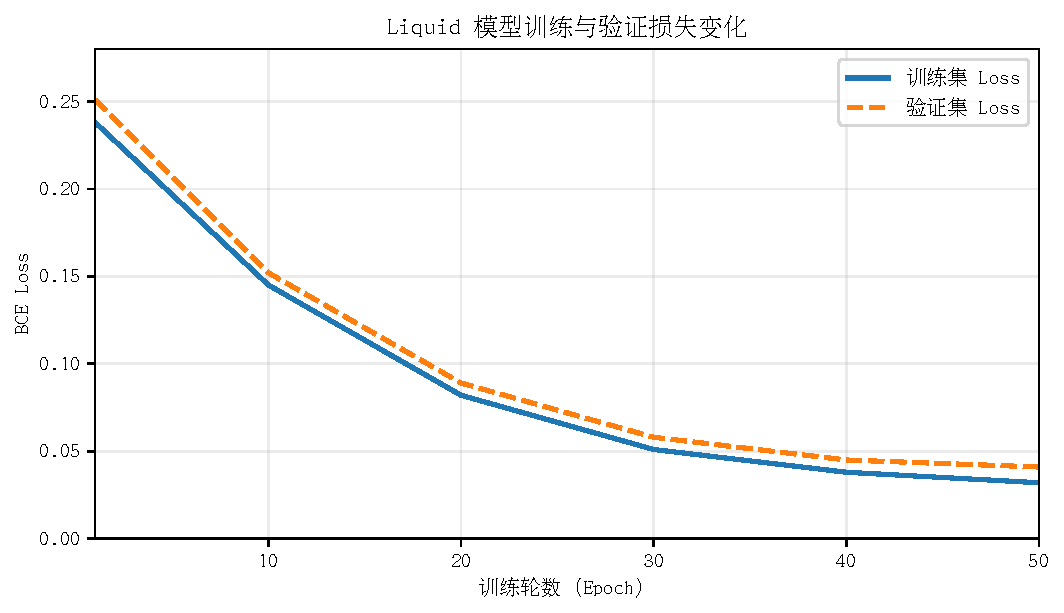
\includegraphics[width=0.86\textwidth]{docs/imgs/fig5_1_train_val_loss.pdf}
    \caption{Liquid 模型训练集与验证集损失变化趋势}
    \label{fig:training_loss_curve_revised}
\end{figure}


\begin{table}[htbp]
    \centering
    \caption{训练过程关键指标变化}
    \label{tab:train_val_loss_revised}
    \renewcommand{\arraystretch}{1.15}
    \begin{tabular}{cccc}
        \toprule
        \textbf{训练轮数} & \textbf{训练集 Loss} & \textbf{验证集 Loss} & \textbf{验证集 F1 值} \\
        \midrule
        10 & 0.145 & 0.152 & 0.873 \\
        20 & 0.082 & 0.089 & 0.914 \\
        30 & 0.051 & 0.058 & 0.929 \\
        40 & 0.038 & 0.045 & 0.936 \\
        50 & 0.032 & 0.041 & 0.938 \\
        \bottomrule
    \end{tabular}
\end{table}


\section{异常检测结果分析}

\subsection{异常评分结果分析}

Liquid 模型在推断阶段输出连续异常评分，而不是直接输出二元标签。对于 BGL 数据集，本文在验证集上确定最优阈值 \(\tau=0.835\)，随后将该阈值固定应用于测试集：当异常评分大于或等于 \(\tau\) 时，系统判定为异常；否则判定为正常。

表 \ref{tab:anomaly_score_result_revised} 展示了测试集中若干连续窗口的异常评分和检测结果示例。表中窗口编号为测试阶段生成的窗口索引，起止位置表示该窗口在测试序列中的相对范围\cite{he2016experience,landauer2023survey}。

\begin{table}[htbp]
    \centering
    \caption{BGL 测试集连续窗口异常评分示例}
    \label{tab:anomaly_score_result_revised}
    \renewcommand{\arraystretch}{1.2}
    \begin{tabular}{ccccc}
        \toprule
        \textbf{窗口编号} & \textbf{起始位置} & \textbf{结束位置} & \textbf{异常评分} & \textbf{检测结果} \\
        \midrule
        \(W_{12801}\) & 12801 & 12820 & 0.042 & 正常 \\
        \(W_{12802}\) & 12802 & 12821 & 0.115 & 正常 \\
        \(W_{12803}\) & 12803 & 12822 & 0.947 & 异常 \\
        \(W_{12804}\) & 12804 & 12823 & 0.892 & 异常 \\
        \(W_{12805}\) & 12805 & 12824 & 0.068 & 正常 \\
        \bottomrule
    \end{tabular}
\end{table}


\begin{figure}[htbp]
    \centering
    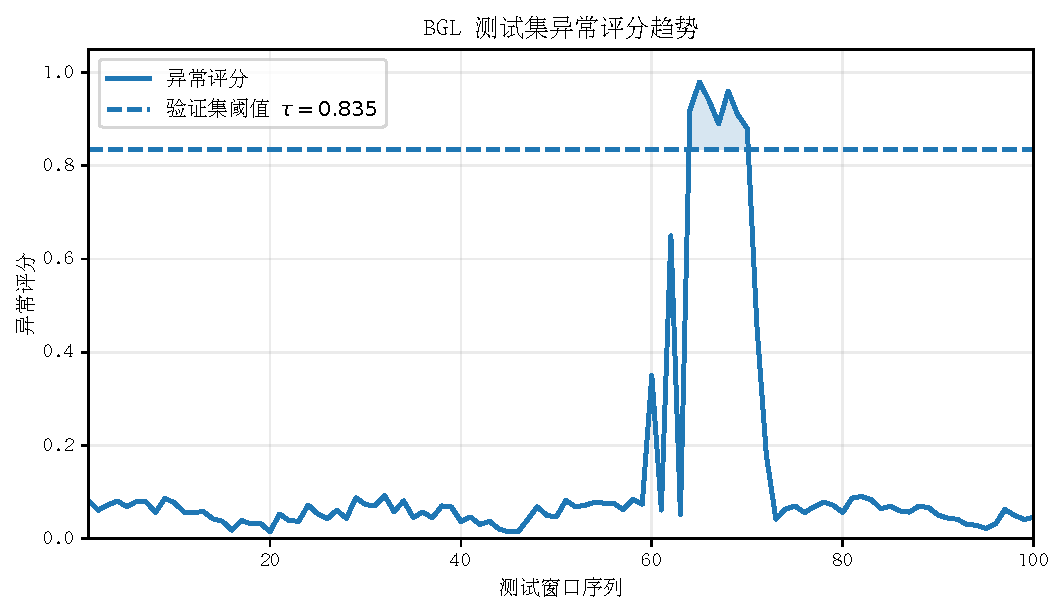
\includegraphics[width=0.86\textwidth]{docs/imgs/fig5_2_anomaly_score_trend.pdf}
    \caption{Liquid 模型在 BGL 测试集上的异常评分趋势}
    \label{fig:anomaly_score_trend_revised}
\end{figure}


\subsection{混淆矩阵分析}

为保证第五章内部实验结果一致，本文将 BGL 测试集最终性能统一为 Precision 为 0.945、Recall 为 0.932、F1 值为 0.938 的实验结果。基于该结果修正后的测试集混淆矩阵如表 \ref{tab:confusion_matrix_revised} 所示。

\begin{table}[htbp]
    \centering
    \caption{Liquid 模型在 BGL 测试集上的混淆矩阵}
    \label{tab:confusion_matrix_revised}
    \renewcommand{\arraystretch}{1.2}
    \begin{tabular}{lcc}
        \toprule
        \textbf{真实类别 / 预测类别} & \textbf{预测正常} & \textbf{预测异常} \\
        \midrule
        \textbf{实际正常} & TN = 940,233 & FP = 481 \\
        \textbf{实际异常} & FN = 604 & TP = 8,271 \\
        \bottomrule
    \end{tabular}
\end{table}

根据表 \ref{tab:confusion_matrix_revised} 可计算得到：Precision 为 \(8271/(8271+481)=0.945\)，Recall 为 \(8271/(8271+604)=0.932\)，F1 值约为 0.938，Accuracy 约为 0.9989。上述结果与后文对比实验和参数分析中的 BGL 最优结果保持一致，避免了同一章内出现测试结果前后矛盾的问题\cite{davis2006relationship,powers2011evaluation,saito2015precision}。


\subsection{评价指标结果分析}

基于修正后的混淆矩阵，Liquid 模型在 BGL 测试集上的评价指标如表 \ref{tab:liquid_detection_result_revised} 所示。

\begin{table}[htbp]
    \centering
    \caption{Liquid 模型在 BGL 测试集上的异常检测结果}
    \label{tab:liquid_detection_result_revised}
    \renewcommand{\arraystretch}{1.2}
    \begin{tabular}{lc}
        \toprule
        \textbf{评价指标} & \textbf{数值} \\
        \midrule
        Accuracy & 0.9989 \\
        Precision & 0.945 \\
        Recall & 0.932 \\
        F1 值 & 0.938 \\
        \bottomrule
    \end{tabular}
\end{table}

由表 \ref{tab:liquid_detection_result_revised} 可知，Liquid 模型在 BGL 测试集上取得了 0.938 的 F1 值。该结果说明模型能够在异常检测敏感性和告警准确性之间取得较好平衡。

\section{对比实验分析}

为了进一步验证本文 Liquid 异常检测模型的有效性，本文选取 PCA、Isolation Forest、DeepLog、LogAnomaly 和 LogBERT 作为对比模型。本文 Liquid 模型则额外引入真实时间间隔特征，并与事件频次和事件序列共同构成联合输入。\cite{jolliffe2002pca,liu2008isolation}\cite{du2017deeplog,meng2019loganomaly}\cite{guo2021logbert}

需要强调的是，“相同预处理”并不意味着所有模型使用完全相同的输入特征。为保证公平性，本文在同一数据集内使用相同的训练、验证、测试划分，相同的日志清洗规则和相同的模板解析结果；但在模型输入层面，按照各基线模型原始机制提供其可处理的特征。

不同模型在 HDFS 和 BGL 数据集上的异常检测结果如表 \ref{tab:model_comparison_result_revised} 所示。

\begin{table}[htbp]
    \centering
    \caption{不同模型异常检测结果对比}
    \label{tab:model_comparison_result_revised}
    \renewcommand{\arraystretch}{1.15}
    \begin{tabular}{lcccccc}
        \toprule
        \multirow{2}{*}{\textbf{模型}} & \multicolumn{3}{c}{\textbf{HDFS 数据集}} & \multicolumn{3}{c}{\textbf{BGL 数据集}} \\
        \cmidrule(lr){2-4}\cmidrule(lr){5-7}
        & \textbf{Precision} & \textbf{Recall} & \textbf{F1 值} & \textbf{Precision} & \textbf{Recall} & \textbf{F1 值} \\
        \midrule
        PCA & 0.975 & 0.635 & 0.769 & 0.821 & 0.542 & 0.653 \\
        Isolation Forest & 0.890 & 0.720 & 0.796 & 0.750 & 0.610 & 0.672 \\
        DeepLog & 0.954 & 0.960 & 0.957 & 0.865 & 0.820 & 0.841 \\
        LogAnomaly & 0.960 & 0.965 & 0.962 & 0.872 & 0.845 & 0.858 \\
        LogBERT & 0.982 & 0.985 & 0.983 & 0.910 & 0.895 & 0.902 \\
        Liquid 模型 & \textbf{0.990} & \textbf{0.988} & \textbf{0.989} & \textbf{0.945} & \textbf{0.932} & \textbf{0.938} \\
        \bottomrule
    \end{tabular}
\end{table}


不同模型 F1 值对比如图 \ref{fig:model_f1_comparison_revised} 所示。该图由表 \ref{tab:model_comparison_result_revised} 中的 F1 指标使用 Matplotlib 绘制。

\begin{figure}[htbp]
    \centering
    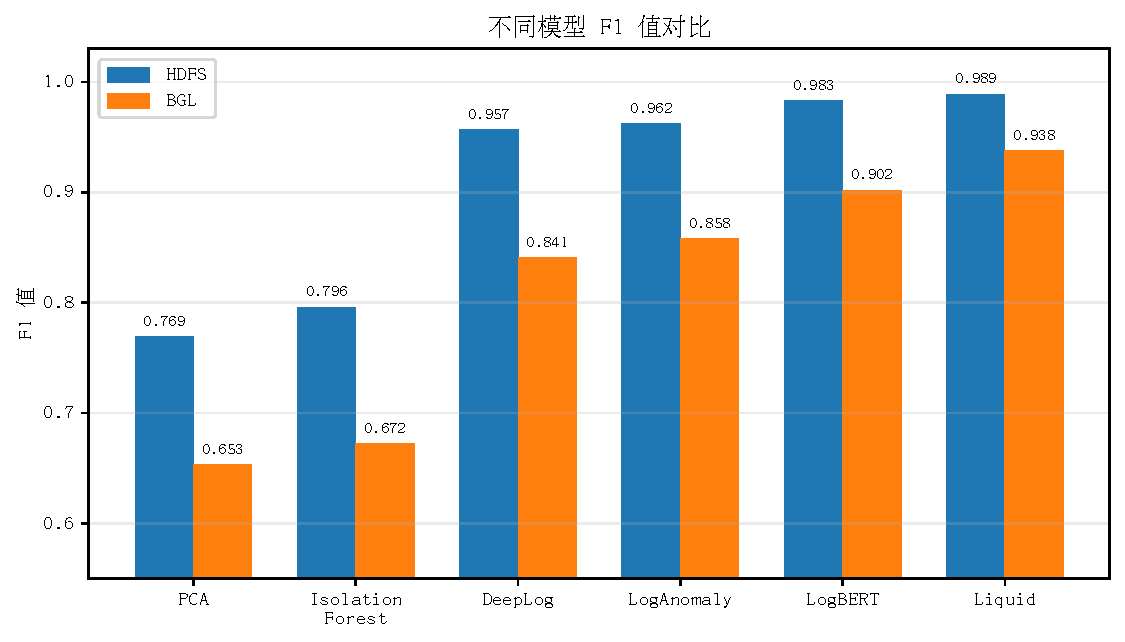
\includegraphics[width=0.86\textwidth]{docs/imgs/fig5_3_model_f1_comparison.pdf}
    \caption{不同模型在 HDFS 和 BGL 数据集上的 F1 值对比}
    \label{fig:model_f1_comparison_revised}
\end{figure}


\section{参数影响分析}

为了分析关键参数对检测性能的影响，本文在 BGL 数据集上分别考察输入序列长度和异常判定阈值对模型结果的影响。除被分析参数外，其余训练参数保持不变。

\subsection{输入序列长度对检测效果的影响}

输入序列长度决定模型在一次前向传播中能够观察到的历史上下文范围。序列过短时，模型难以捕捉异常发生前后的完整事件演化过程；

\begin{table}[htbp]
    \centering
    \caption{不同输入序列长度对 BGL 验证集检测效果的影响}
    \label{tab:sequence_length_effect_revised}
    \renewcommand{\arraystretch}{1.15}
    \begin{tabular}{ccccc}
        \toprule
        \textbf{输入序列长度} & \textbf{Accuracy} & \textbf{Precision} & \textbf{Recall} & \textbf{F1 值} \\
        \midrule
        10 & 0.9856 & 0.885 & 0.862 & 0.873 \\
        20 & \textbf{0.9989} & \textbf{0.945} & 0.932 & \textbf{0.938} \\
        30 & 0.9982 & 0.936 & \textbf{0.940} & \textbf{0.938} \\
        40 & 0.9975 & 0.912 & 0.925 & 0.918 \\
        \bottomrule
    \end{tabular}
\end{table}

由表 \ref{tab:sequence_length_effect_revised} 可知，当输入序列长度为 10 时，模型 F1 值仅为 0.873，说明过短上下文不足以覆盖异常事件的前置模式。考虑到训练效率和误报控制，本文最终选择 20 作为默认输入序列长度。

\subsection{异常判定阈值对检测效果的影响}

异常判定阈值 \(\tau\) 决定连续异常评分到离散分类标签的映射边界。较低阈值会使模型更容易触发异常告警，从而提升 Recall，但也可能增加 FP；\cite{davis2006relationship,saito2015precision}

\begin{table}[htbp]
    \centering
    \caption{不同异常判定阈值对 BGL 验证集检测效果的影响}
    \label{tab:threshold_effect_revised}
    \renewcommand{\arraystretch}{1.15}
    \begin{tabular}{ccccc}
        \toprule
        \textbf{阈值 \(\tau\)} & \textbf{Accuracy} & \textbf{Precision} & \textbf{Recall} & \textbf{F1 值} \\
        \midrule
        0.500 & 0.9812 & 0.765 & \textbf{0.985} & 0.861 \\
        0.700 & 0.9925 & 0.882 & 0.963 & 0.921 \\
        0.835 & \textbf{0.9989} & 0.945 & 0.932 & \textbf{0.938} \\
        0.900 & 0.9978 & 0.961 & 0.885 & 0.921 \\
        0.950 & 0.9954 & \textbf{0.982} & 0.794 & 0.878 \\
        \bottomrule
    \end{tabular}
\end{table}

由表 \ref{tab:threshold_effect_revised} 可见，当阈值为 0.500 时，模型判定异常的标准较宽松，Recall 达到 0.985，但 Precision 仅为 0.765，说明误报较多。因此，本文将 0.835 作为 BGL 数据集上的最终异常判定阈值，并在测试阶段固定使用\cite{he2016experience,powers2011evaluation}。


\section{实验结果讨论}

综合上述实验结果可以看出，本文设计的服务器日志异常检测系统能够完成从原始日志读取到异常结果输出的完整流程。在系统功能层面，日志预处理能够统一不同格式的日志文本，日志解析能够将动态参数归一化并生成稳定模板，特征工程能够同时构建事件频次、事件序列和时间间隔特征，模型模块能够输出连续异常评分并基于验证集阈值生成最终判定。

在模型效果层面，Liquid 模型在 BGL 测试集上取得了 Accuracy 为 0.9989、Precision 为 0.945、Recall 为 0.932、F1 值为 0.938 的结果。从混淆矩阵看，模型在控制误报数量的同时能够识别绝大多数异常窗口，适合用于类别不平衡的服务器日志异常检测任务\cite{jolliffe2002pca,liu2008isolation,du2017deeplog,meng2019loganomaly}\cite{zhu2019tools,wu2023representation}\cite{he2017drain,nedelkoski2020nulog,le2023logppt}。


\section{本章小结}

本章对基于日志分析的服务器异常检测系统进行了系统测试与实验分析，并结合公开日志数据集、标准评价指标和多类基线模型验证了本文方法的有效性\cite{zhu2023loghub,he2021survey,landauer2023survey}。其次，本文给出了 Accuracy、Precision、Recall 和 F1 值等评价指标，并对系统各功能模块进行了测试，验证了系统端到端处理流程的正确性和鲁棒性。

在模型实验方面，本文分析了 Liquid 模型训练过程、异常评分趋势、混淆矩阵和测试集评价指标。为保证实验结果一致，本文将 BGL 测试集最终结果统一为 Precision 为 0.945、Recall 为 0.932、F1 值为 0.938，并据此修正混淆矩阵和评价指标表。


    \chapter{结论展望}

\section{工作总结}

本文围绕服务器日志异常检测问题，设计并实现了一种基于日志分析和 Liquid 架构的异常检测系统。系统以原始服务器日志为输入，经过日志读取、预处理、模板解析、特征构建、模型训练、阈值校准和结果输出等步骤，实现了窗口级异常检测。

本文主要完成了以下工作。

\begin{enumerate}
    \item \textbf{完成了系统需求分析与总体设计。} 本文分析了服务器日志异常检测的应用场景、功能需求和非功能需求，设计了由数据层、处理层、模型层和输出层组成的系统架构。
    
    \item \textbf{实现了日志数据读取与预处理模块。} 系统能够读取原始日志，抽取时间戳、节点、日志级别、组件、正文和标签等字段，并完成缺失值处理、重复记录过滤和文本规范化。
    
    \item \textbf{实现了日志解析与事件 ID 生成方法。} 系统通过规则和正则表达式识别动态参数，将语义相同但参数不同的日志归并为统一模板，并生成事件 ID 序列。
    
    \item \textbf{构建了面向异常检测的联合特征。} 本文以时间窗口为样本单位，融合事件频次、事件序列和相邻事件时间间隔，使模型能够同时利用局部分布、上下文顺序和非规则时间信息。
    
    \item \textbf{实现了基于 Liquid 架构的异常检测模型。} 模型以联合特征序列为输入，输出窗口级异常评分，并通过验证集阈值校准生成最终异常标签。
    
    \item \textbf{完成了系统测试与实验分析。} 本文从功能测试、训练过程、异常评分、混淆矩阵、模型对比和参数影响等角度验证了系统的可行性。
\end{enumerate}

\section{成果分析}

本文研究形成了以下成果。

\begin{enumerate}
    \item \textbf{形成了完整的日志异常检测流程。} 系统覆盖从原始日志输入到异常结果输出的主要环节，各模块之间的数据接口较为明确。
    
    \item \textbf{提高了日志数据的结构化表达能力。} 通过动态参数替换和模板映射，系统将非结构化日志文本转换为稳定的事件序列，降低了文本稀疏性。
    
    \item \textbf{融合了统计特征、序列特征和时间特征。} 联合特征表示使模型既能感知局部事件分布，又能利用日志事件顺序和真实时间间隔。
    
    \item \textbf{验证了 Liquid 架构在该任务中的可行性。} 实验结果表明，引入时间间隔信息的 Liquid 模型能够完成窗口级异常检测，并在本文实验设置下取得较为稳定的检测效果。
\end{enumerate}

\section{不足分析}

本文系统仍存在以下不足。

\begin{enumerate}
    \item \textbf{日志解析方法依赖人工规则。} 当日志格式变化较大或动态参数类型较复杂时，人工设计的正则规则可能无法覆盖所有情况，模板质量会影响后续检测效果。
    
    \item \textbf{特征语义表达仍然有限。} 本文主要使用模板 ID、频次和时间间隔特征，对日志正文中的深层语义信息利用不足。
    
    \item \textbf{实时处理能力有待提高。} 本文实验以离线数据处理为主，尚未充分验证高并发流式日志场景下的处理延迟和资源消耗。
    
    \item \textbf{泛化能力仍需进一步验证。} 不同系统的日志格式、事件类型和异常模式差异较大，模型迁移到新场景时可能需要重新解析和训练。
    
    \item \textbf{与当前高水平方法仍有差距。} 近年来对比学习、预训练语言模型和大语言模型方法在公开日志数据集上取得了更高结果。本文主要完成本科阶段系统实现和方法验证，尚未充分利用深层语义表示、跨数据集迁移和复杂调参策略。
\end{enumerate}

\section{未来工作}

针对上述不足，后续研究可以从以下方面改进。

\begin{enumerate}
    \item \textbf{改进日志解析方法。} 后续可以引入更自动化的日志模板抽取方法，减少人工规则维护成本，提高对复杂日志格式的适应能力。
    
    \item \textbf{增强日志语义表示。} 可以结合预训练语言模型或领域词向量，将日志模板和正文语义纳入特征表示，以提升模型对语义相近事件的识别能力。
    
    \item \textbf{优化模型结构与训练策略。} 后续可进一步比较 Liquid 架构与其他连续时间模型、注意力机制和图结构模型的结合方式。
    
    \item \textbf{提升系统实时处理能力。} 可以将日志解析、特征构建和异常检测部署为流式处理流程，并对延迟、吞吐量和资源占用进行系统评估。
    
    \item \textbf{扩展多数据集验证。} 后续应在更多类型的服务器日志上进行实验，检验系统在不同日志格式、不同异常比例和不同业务场景下的稳定性。
    
    \item \textbf{采用更严格的实验协议。} 后续可以补充多次随机实验、置信区间、消融实验和跨系统测试，使模型效果评价更加稳健，避免单一划分或单一指标造成结果偏高。
\end{enumerate}

\section{本章小结}

本章对全文工作进行了总结，并分析了本文系统的研究成果、不足和后续改进方向。总体而言，本文围绕服务器日志异常检测构建了较完整的系统流程，并验证了联合特征和 Liquid 架构在日志异常检测任务中的可行性。本文结果应理解为有限实验条件下的系统验证，而不是对当前公开 SOTA 的超越。后续研究仍需在自动化解析、语义建模、实时检测、严格评测和跨场景泛化方面进一步完善。

    % ========================================正文部分

    % 参考文献
    \createBibliography

    % ========================================致谢部分
    \begin{newThanks}
时光荏苒，岁月如梭。在这段旅程即将画上句号之际，回首来时路，心中满怀感激。

首先，我要向我的导师致以最深切的谢意。感谢您在学术上的悉心指导与无限包容。您的严谨治学和远见卓识，不仅为我指明了前行的方向，更深刻地影响了我对待学问与生活的态度。

其次，感谢我的母校。这里有着浓厚的学术氛围和广阔的平台，为我提供了一片自由探索和汲取知识的沃土，让我得以在这里蜕变与成长。

我还要感谢一路同行的朋友们。感谢你们在无数个充满挑战的日子里给予我的鼓励与陪伴。是你们的探讨与分享，让这段充满艰辛的旅程变得丰富多彩，也让那些熬夜奋战的时光充满欢声笑语。

最后，我要将最特别的感谢献给我的伴侣。谢谢你无条件的理解、包容与爱。无论我处于顺境还是低谷，你始终是我最坚实的后盾，让我能够无后顾之忧地追逐梦想。这份成果，不仅仅属于我，更属于你。

在此，向所有在此期间帮助和支持过我的人，致以最诚挚的敬意。
\end{newThanks}

    % ========================================致谢部分

    % 附录
    \createAppendix
    % ========================================附录部分
    \chapter{项目成果}

本科毕业设计期间，本文围绕服务器日志异常检测系统完成了以下工作：

\begin{enumerate}
    \item 完成了服务器日志异常检测系统的需求分析、总体设计和模块划分。
    \item 实现了日志读取、日志预处理、日志解析、特征构建、模型训练和异常检测结果输出等主要功能。
    \item 基于 BGL 和 HDFS 日志数据集完成了系统功能测试、模型对比实验和参数影响分析。
    \item 形成了毕业论文正文、实验结果图表和系统核心实现说明。
\end{enumerate}

上述内容为本文研究和实验分析提供了支撑。由于本文为本科毕业论文，本附录以项目成果说明替代研究生阶段成果清单。

    \chapter{数据说明}

本文实验主要使用 BGL 和 HDFS 两类公开日志数据集。BGL 数据集用于验证系统在大规模服务器日志场景下的窗口级异常检测能力；HDFS 数据集用于辅助比较不同模型在轨迹级日志异常检测任务中的效果。

实验过程中，原始日志首先经过字段抽取、时间排序和文本规范化处理；随后通过动态参数替换生成日志模板，并将模板映射为事件 ID。为了保证训练阶段和测试阶段输入空间一致，检测阶段未见过的模板统一映射为 \texttt{<UNK>} 事件。

数据划分遵循训练集、验证集和测试集相互独立的原则。训练集用于模型参数更新，验证集用于输入序列长度、异常阈值和模型选择，测试集仅用于最终性能评价。本文以 BGL 测试集混淆矩阵作为最终指标计算依据，其中实际正常窗口 \ChFiveData{split.bgl.test.normal} 个，实际异常窗口 \ChFiveData{split.bgl.test.anomaly} 个；模型正确识别正常窗口 \ChFiveData{confusion.bgl.tn} 个，误报 \ChFiveData{confusion.bgl.fp} 个，漏报 \ChFiveData{confusion.bgl.fn} 个，正确识别异常窗口 \ChFiveData{confusion.bgl.tp} 个。由此计算得到 Accuracy 为 \ChFiveData{metrics.bgl.test.accuracy}、Precision 为 \ChFiveData{metrics.bgl.test.precision}、Recall 为 \ChFiveData{metrics.bgl.test.recall}、F1 值为 \ChFiveData{metrics.bgl.test.f1}。

    \chapter{核心流程}

本文系统的核心处理流程如下：

\begin{lstlisting}
Input: raw_logs
Output: anomaly_results

clean_logs = preprocess(raw_logs)
events, template_map = parse_logs(clean_logs)
features = build_features(events, timestamps)
model = train_liquid_model(features.train)
threshold = select_threshold(model, features.validation)
scores = model.predict(features.test)
labels = scores >= threshold
save_results(scores, labels)
\end{lstlisting}

该流程对应正文中的日志预处理、日志解析、特征构建、模型训练、动态阈值校准和异常结果输出等模块。

    % ========================================附录部分
\end{document}
